\section{Signal Modeling} \label{section:higgs_signalmodel}
%
% General Description
%
To be able to draw conclusions about possible excess of events, due to the Standard Model Higgs Boson, we ought to build a model aiming to explain the to be observed excess. Given we are looking for a bump-like structure near the Higgs Boson Mass, it is natural to model this excess via a composition of Gaussian functions. Each category and production process has been treated individually and only depends on the Higgs Boson Mass and nuisance parameters to be described further in the section~\ref{section:higgs_signal_systematics}.

Both double eq~\ref{eq:DoubleGaus} and triple eq~\ref{eq:TripleGaus} Gaussian forms were tested. The main reason for extending the form up to triple Gaussian (w.r.t. Run~I) is to be able to pick up both the possible mass shift due to Finite State Radiation (FSR) and accomodate the broadening due to detector resolution effects. Moreover, triple Gaussian form is defined using recursive coefficients to make sure that there are no negative contributions from any of the gaussians.
\begin{align}
   \label{eq:DoubleGaus}
   S(x,\mH, \theta) &= f \mathcal{N}_{1}(x, \mu_{1}, \sigma_{1}) + (1-f)  \mathcal{N}_{2}(x, \mu_{2}, \sigma_{2}) \\
   \label{eq:TripleGaus}
   S(x,\mH, \theta) &= f_{1} \mathcal{N}_{1}(x, \mu_{1}, \sigma_{1}) + (1-f_{1}) \left(f_{2} \mathcal{N}_{2}(x, \mu_{2}, \sigma_{2}) + (1-f_{2}) \mathcal{N}_{3}(x, \mu_{3}, \sigma_{3})\right)
\end{align}

where $\mathcal{N}(x,0,1)$ is a normal distribution, $\mu_i(\mH,\theta), \sigma_i(\mH,\theta)$ are respectively the mean and sigma of each gaussian, $x$ is the reconstructed invariant mass of the two muons (\mmm), and $\theta$ is the list of parametric nuisances.

For each category and each production process (ggH, qqH, WPlusH, WMinusH, ZH, ttH) , all of the signal parameters are derived by fitting a given model (Double eq~\ref{eq:DoubleGaus} or Triple eq~\ref{eq:TripleGaus} Gaus) to the dimuon invariant mass spectrum obtained from the MC Higgs signal samples being subject to the same event selection as data and the same categorization procedure. Note, that in this section, we will discuss the results and show distributions for the Greedy Categorization procedure, however the same applies to the baseline algorithm.

For the purpose of testing various Higgs Boson Mass hypotheses, three mass points ($\mH=120\,\gev$, $125\,\gev$, $130\,\gev$) were used, which allow us to interpolate in between and probe any mass in the range $[120, 130]\,\gev$. The procedure to extract model parameters from the signal MC goes as following:
\begin{itemize}
    \item For a given category and production process
    \item Start with the invariant mass spectrum for $\mH$ of $120\,\gev$ and perform a binned maximum likelihood fit using initial default parameters.
    \item Proceed to next point in mass ($\mH$ of 125 GeV), by using the same fitted resolution ($\sigma_{i}$) from the previous fit ($\mH= 120\gev$) and shifted scale ($\mu_{i}$), by the mass difference, parameters as initial guesses. Perform the Maxlikelihood Fit again and extract the parameters.
    \item Proceed to the $\mH$ of $130\,\gev$ and perform the same procedure as for $125\,GeV$.
    \item This procedure can be applied to any number of mass points.
    \item Each parameter $\mu_{i}, \sigma_{i}, f_{i}$ can be now interpolated across the mass points, using a spline function.
    \item At this point, we have all the parameters ($\sigma_{i}$, $\mu_{i}$, $f_{i}$) as functions of $\mH$.
\end{itemize}

Figure~\ref{fig:higgs_signalmodel_c12gluglu120125130} shows examples of the individual fits of different Higgs Boson mass hypotheses for the most sensitive category,  ''c12'' with the dominant Higgs Boson production mechanism, Gluon Fusion. In both cases, we do not normalize the functional form to the expected yield at 36 fb$^{-1}$ at this stage.
 \begin{figure}[H]
     \centering
     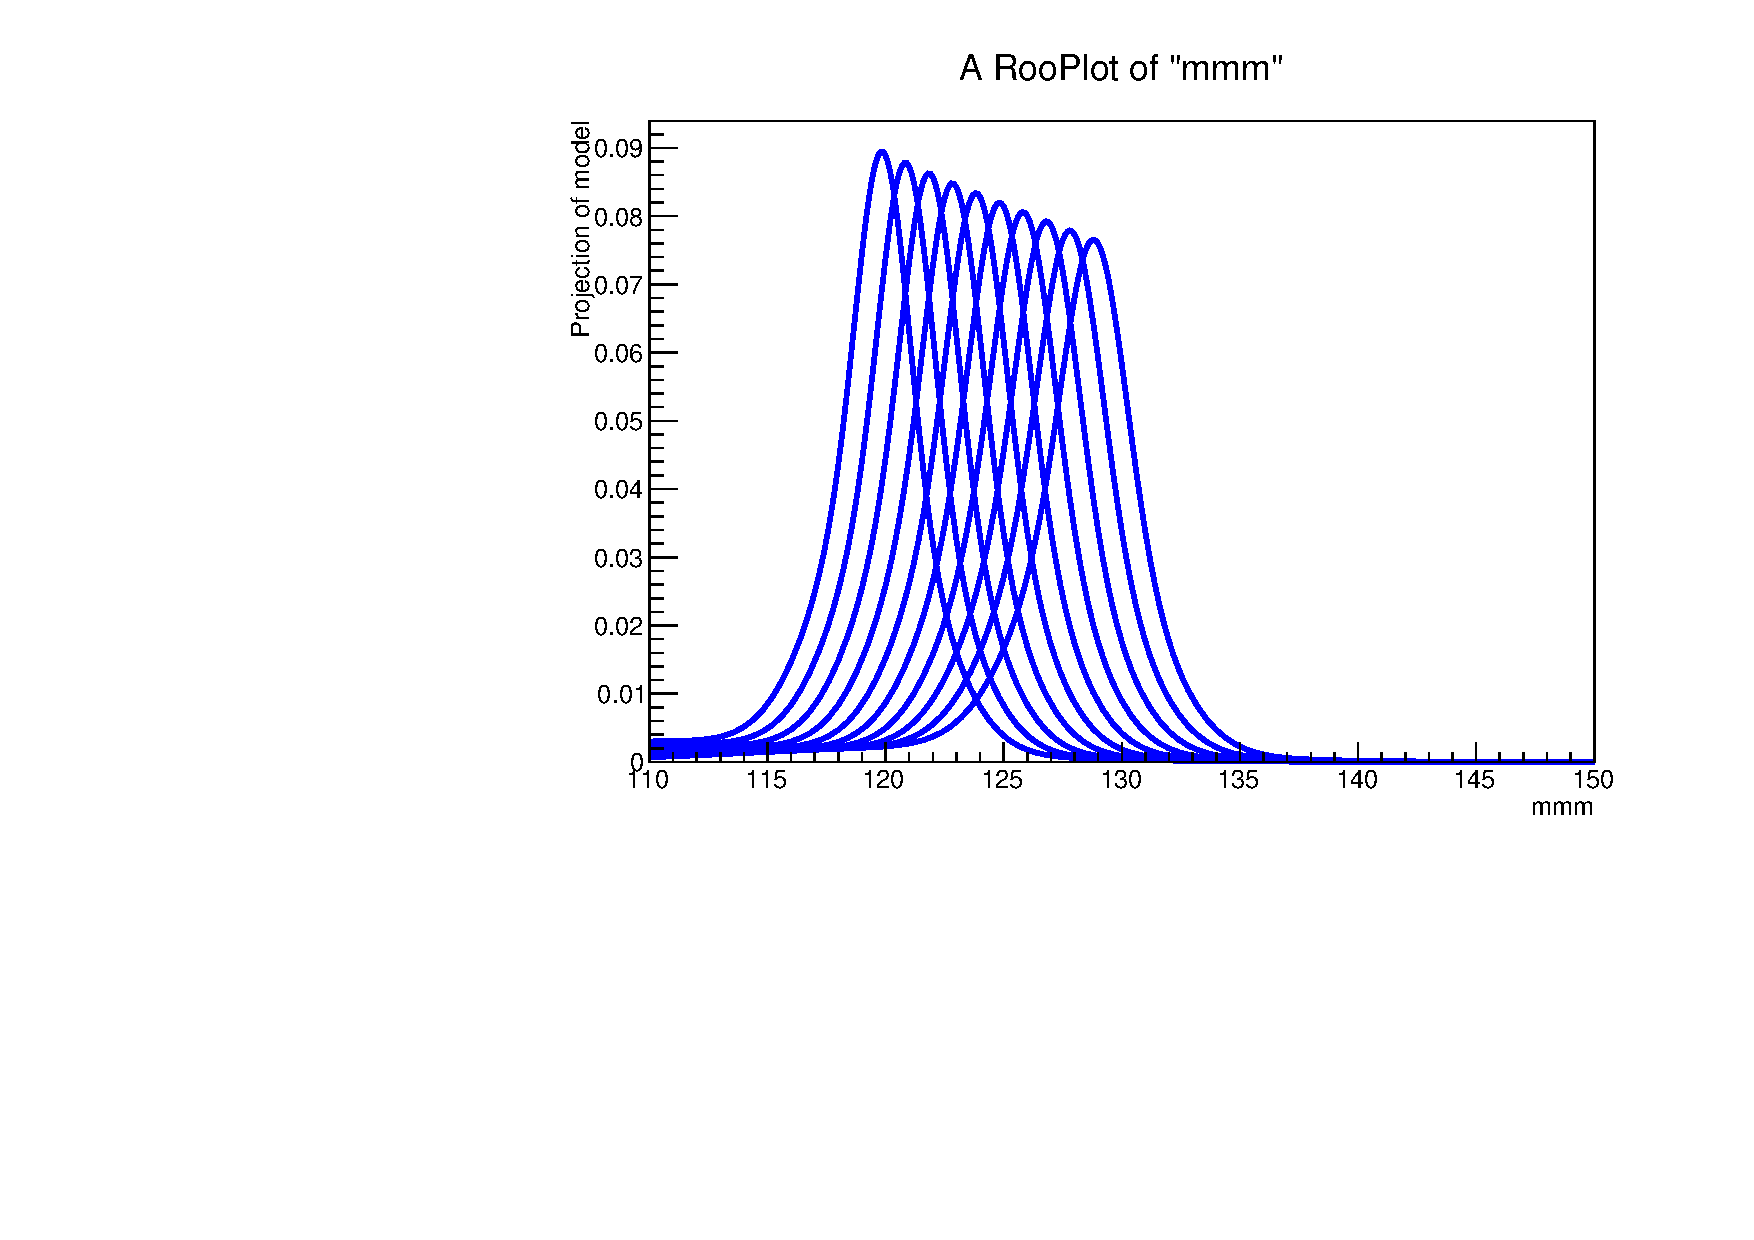
\includegraphics[width=0.8\textwidth]{figures/signal_model/AppendixBdt/interpolation_GluGlu_cat12.pdf}
     \caption{Example of the results of the Signal Interpolation for the Gluon Fusion production mechanism for the most sensitive category, ''c12''}
     \label{fig:higgs_signalmodel_c12glugluinterp}
 \end{figure}
 \begin{figure}[hbp]
     \centering
     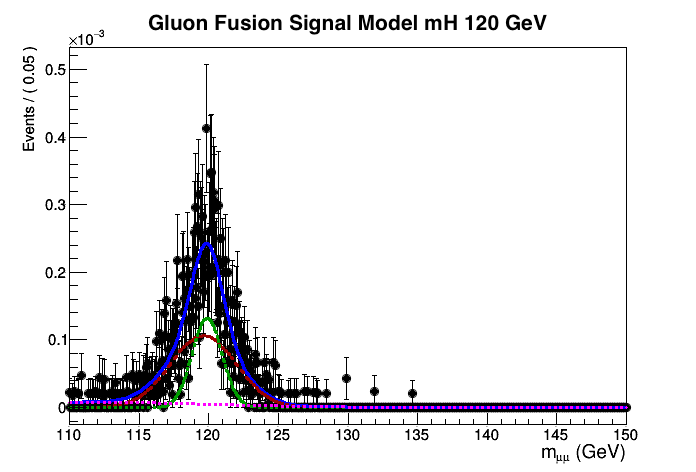
\includegraphics[width=0.65\textwidth]{figures/signal_model/AppendixBdt/GluGlu/120/fit_mh_120_GluGlu_cat12.png}\\
     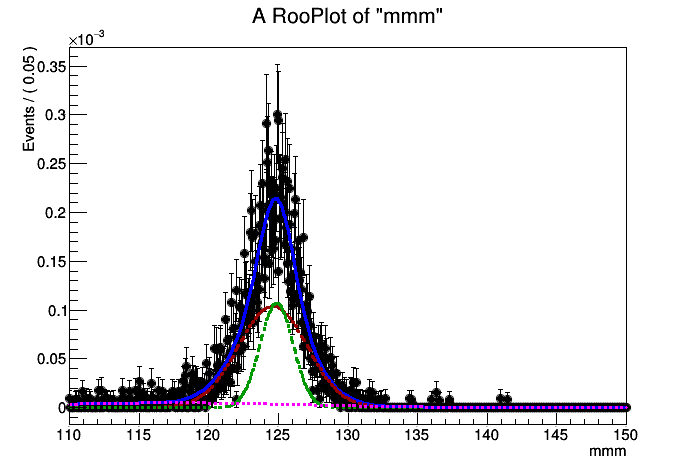
\includegraphics[width=0.65\textwidth]{figures/signal_model/AppendixBdt/GluGlu/125/fit_mh_125_GluGlu_cat12.png}\\
     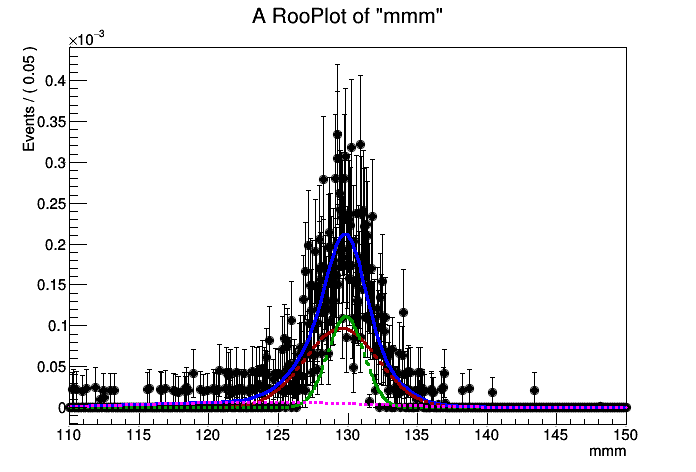
\includegraphics[width=0.65\textwidth]{figures/signal_model/AppendixBdt/GluGlu/130/fit_mh_130_GluGlu_cat12.png}
     \caption{Examples of fits for the individual dimuon mass distributions of signal MC for the Gluon Fusion production mechanism for the most sensitive category, ''c12''. 120 GeV signal (Top), 125 GeV (Middle), and 130 GeV (Bottom)}
     \label{fig:higgs_signalmodel_c12gluglu120125130}
 \end{figure}

The last missing piece for our signal model construction is the normalization. Given a dimuon invariant mass distribution for a particular category for a particular production process, the expected yields can be expressed as in equation~\ref{eq:expectedYield}.
\begin{align}
        %\label{eq:signalNormalization}
        %\text{Norm} = {\frac{\mathcal{L} \sigma \mathcal{B}(\Htomm)}{N_{gen}}} \\
        \label{eq:expectedYield}
        %\text{Yield} = {Norm \times \sum_{bins}^{} N_{i}}
        %\label{eq:efficienceAcceptance}
        \text{Yield} = \mathcal{L}\,\sigma(pp\rightarrow H)\, \mathcal{B}(\Htomm) \, \varepsilon A
\end{align}

The production cross sections ($\sigma(pp\rightarrow H+X)$) for each process and the branching ratio of the Higgs boson to decay into a muon pair ($\mathcal{B}(\Htomm)$) are taken from the Yellow~Report~4 \cite{YR4} as centrally provided by the CMS Higgs Combination Group (see more on this in section~\ref{combine_tool}). Effieciency times acceptance ($\varepsilon A$) is computed using the MC sample information as
\begin{align}
\varepsilon A = \frac{1}{N}\sum w_i r_{i} \text{sf}_i \mathbf{1}_\textup{catX}
\end{align}

where $w_i$ is the generator weight, $r_i$ is the ``pileup reiweighting'' factor used to match the truth pu distribution injected in the MC to the one measured in data, $\text{sf}_i$ is the total scale factor associated to the event,$\mathbf{1}_\textup{catX}$ is the identity function on the classification ($1$ if the event is in the category, $0$ otherwise), and $N$ is the total normalization factor at generator level $N=\sum w_i$, where the sums runs over the entire MC dataset.

Finally, figures~\ref{fig:higgs_signalmodel_gluvbfc0c2}-~\ref{fig:higgs_signalmodel_gluvbfc9c11} show the results of the interpolation algorithm for the 2 dominant Higgs Boson production processes for all of the categories (skipped ''c12''): Vector Boson Fusion and Gluon Fusion.
\begin{figure}[hbp]
  \centering
  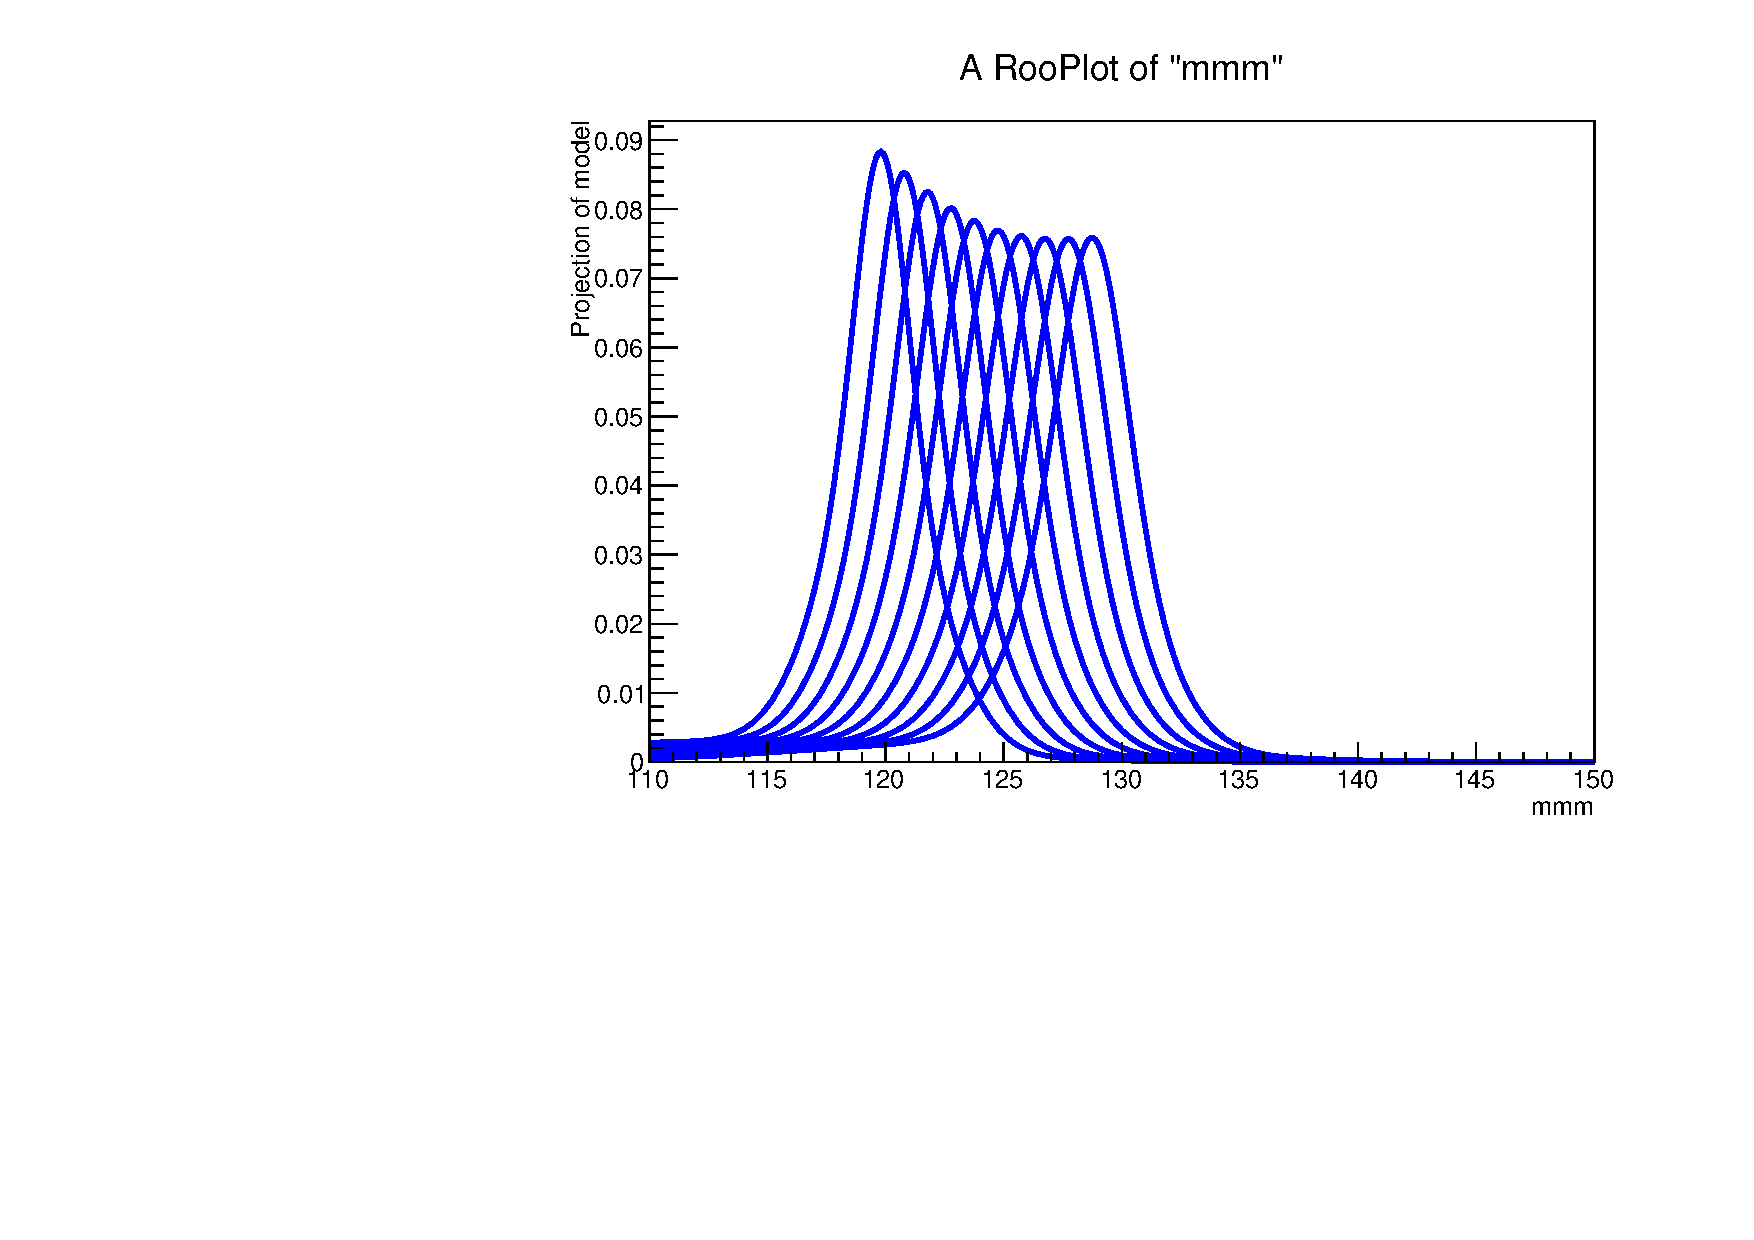
\includegraphics[width=0.49\linewidth]{figures/signal_model/AppendixBdt/interpolation_GluGlu_cat0.pdf}
  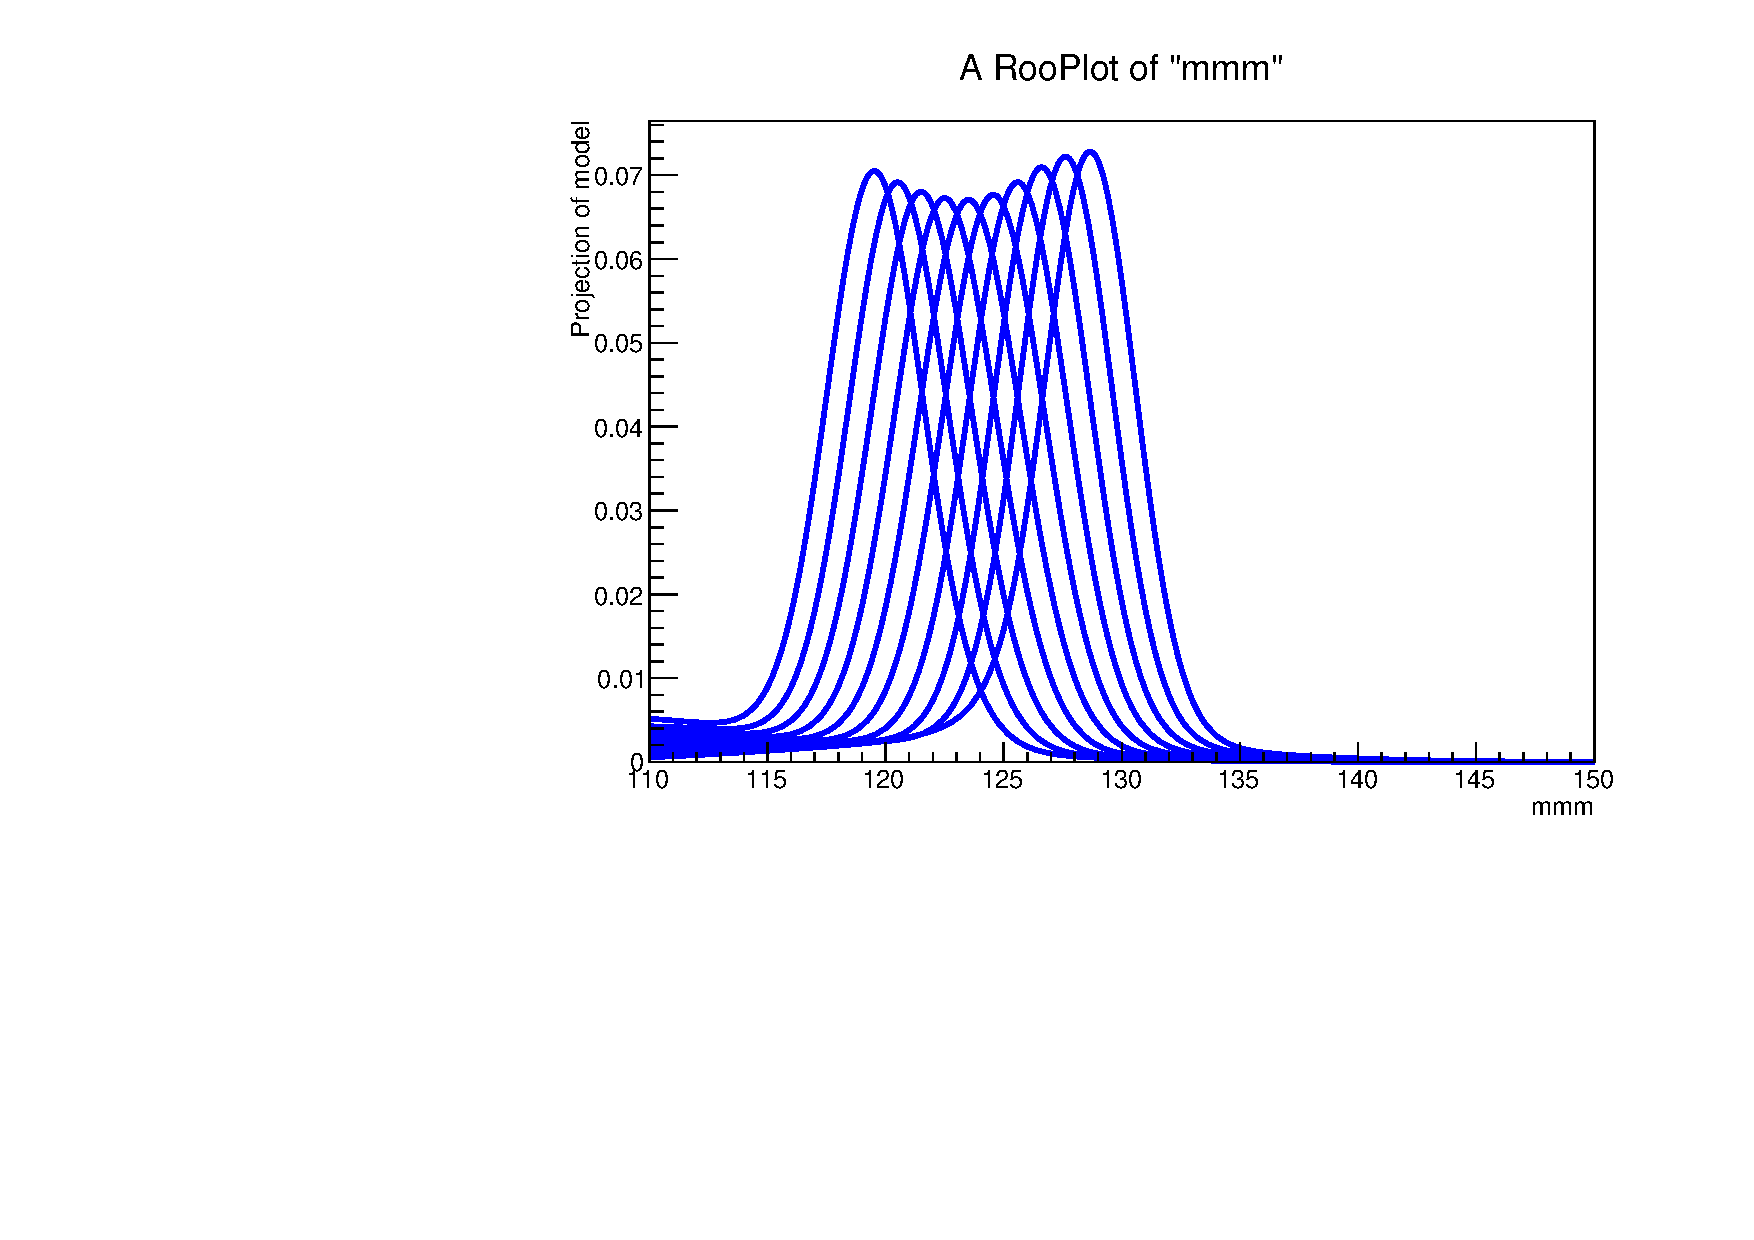
\includegraphics[width=0.49\linewidth]{figures/signal_model/AppendixBdt/interpolation_VBF_cat0.pdf}\\
  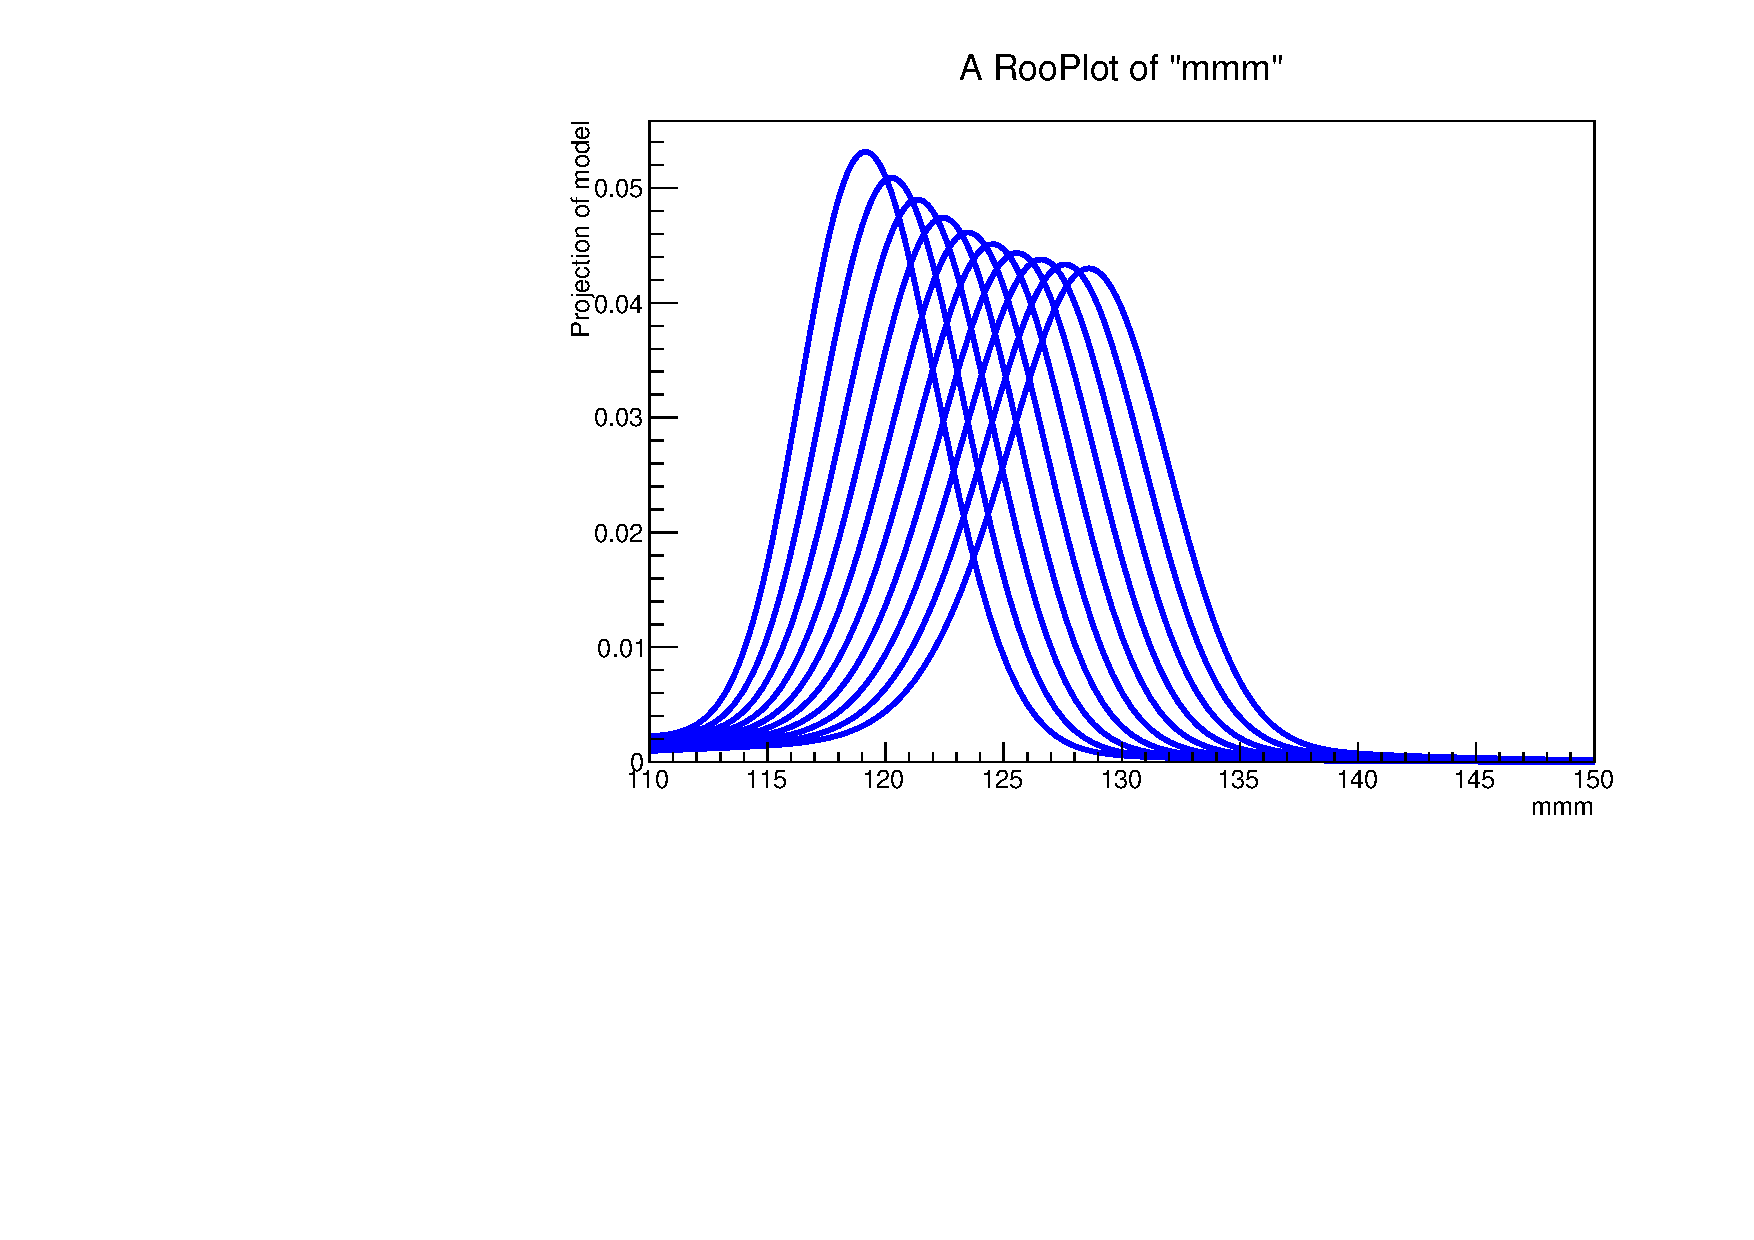
\includegraphics[width=0.49\linewidth]{figures/signal_model/AppendixBdt/interpolation_GluGlu_cat1.pdf}
  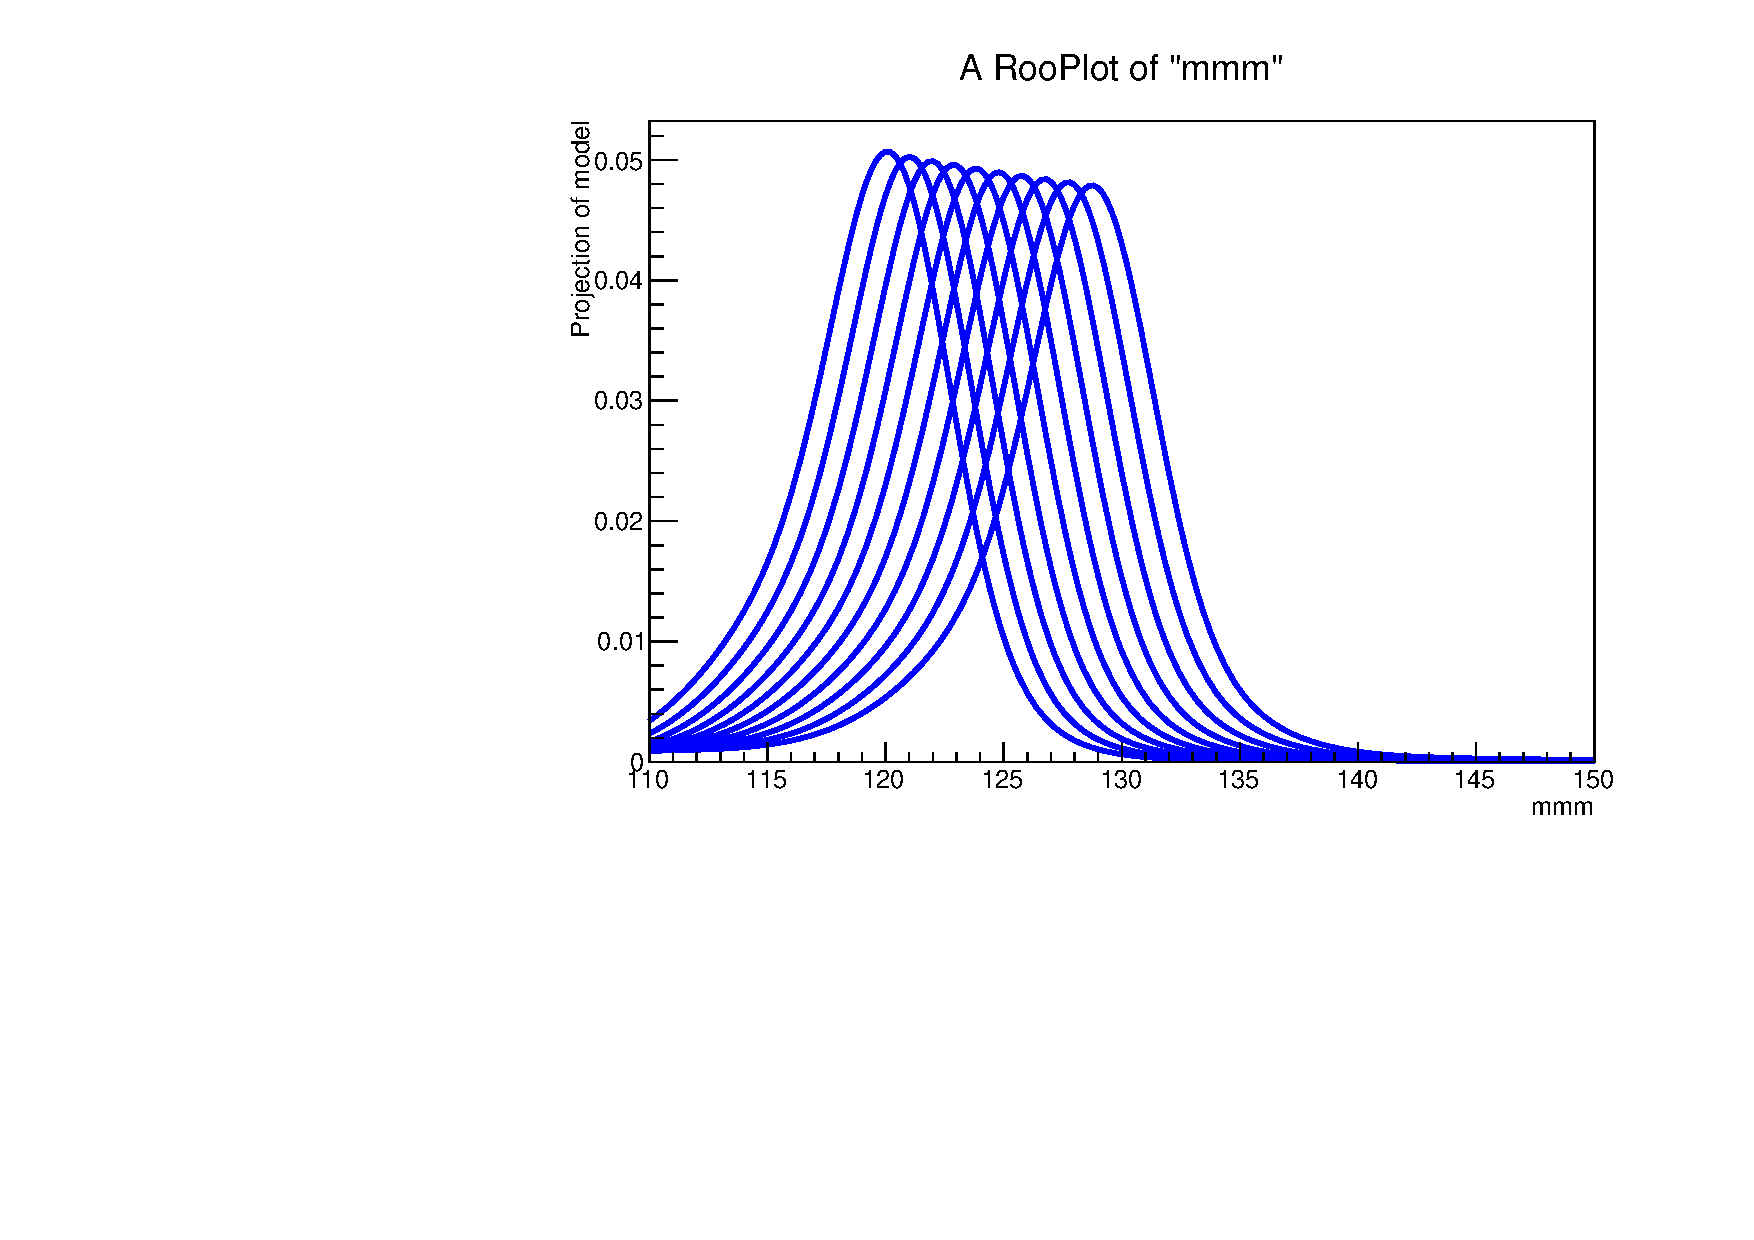
\includegraphics[width=0.49\linewidth]{figures/signal_model/AppendixBdt/interpolation_VBF_cat1.pdf}\\
  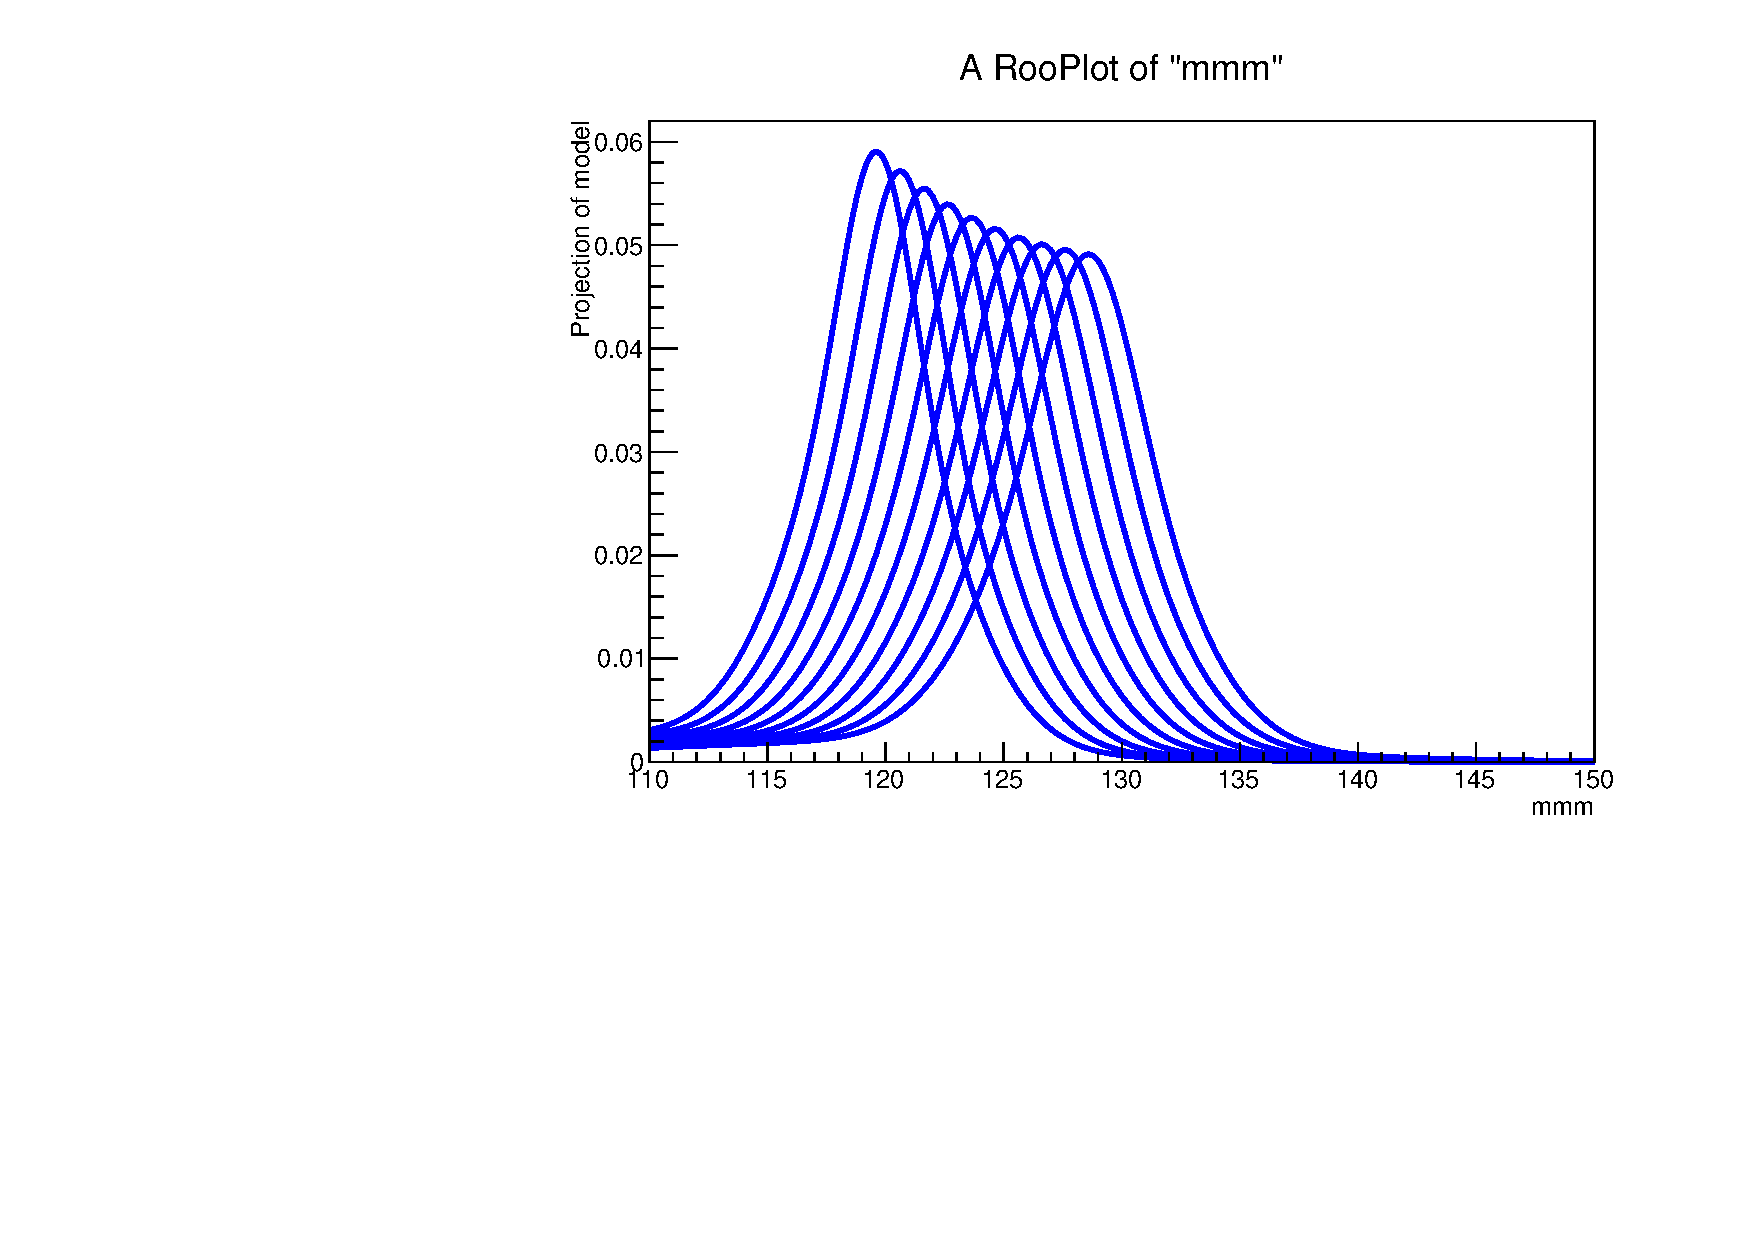
\includegraphics[width=0.49\linewidth]{figures/signal_model/AppendixBdt/interpolation_GluGlu_cat2.pdf}
  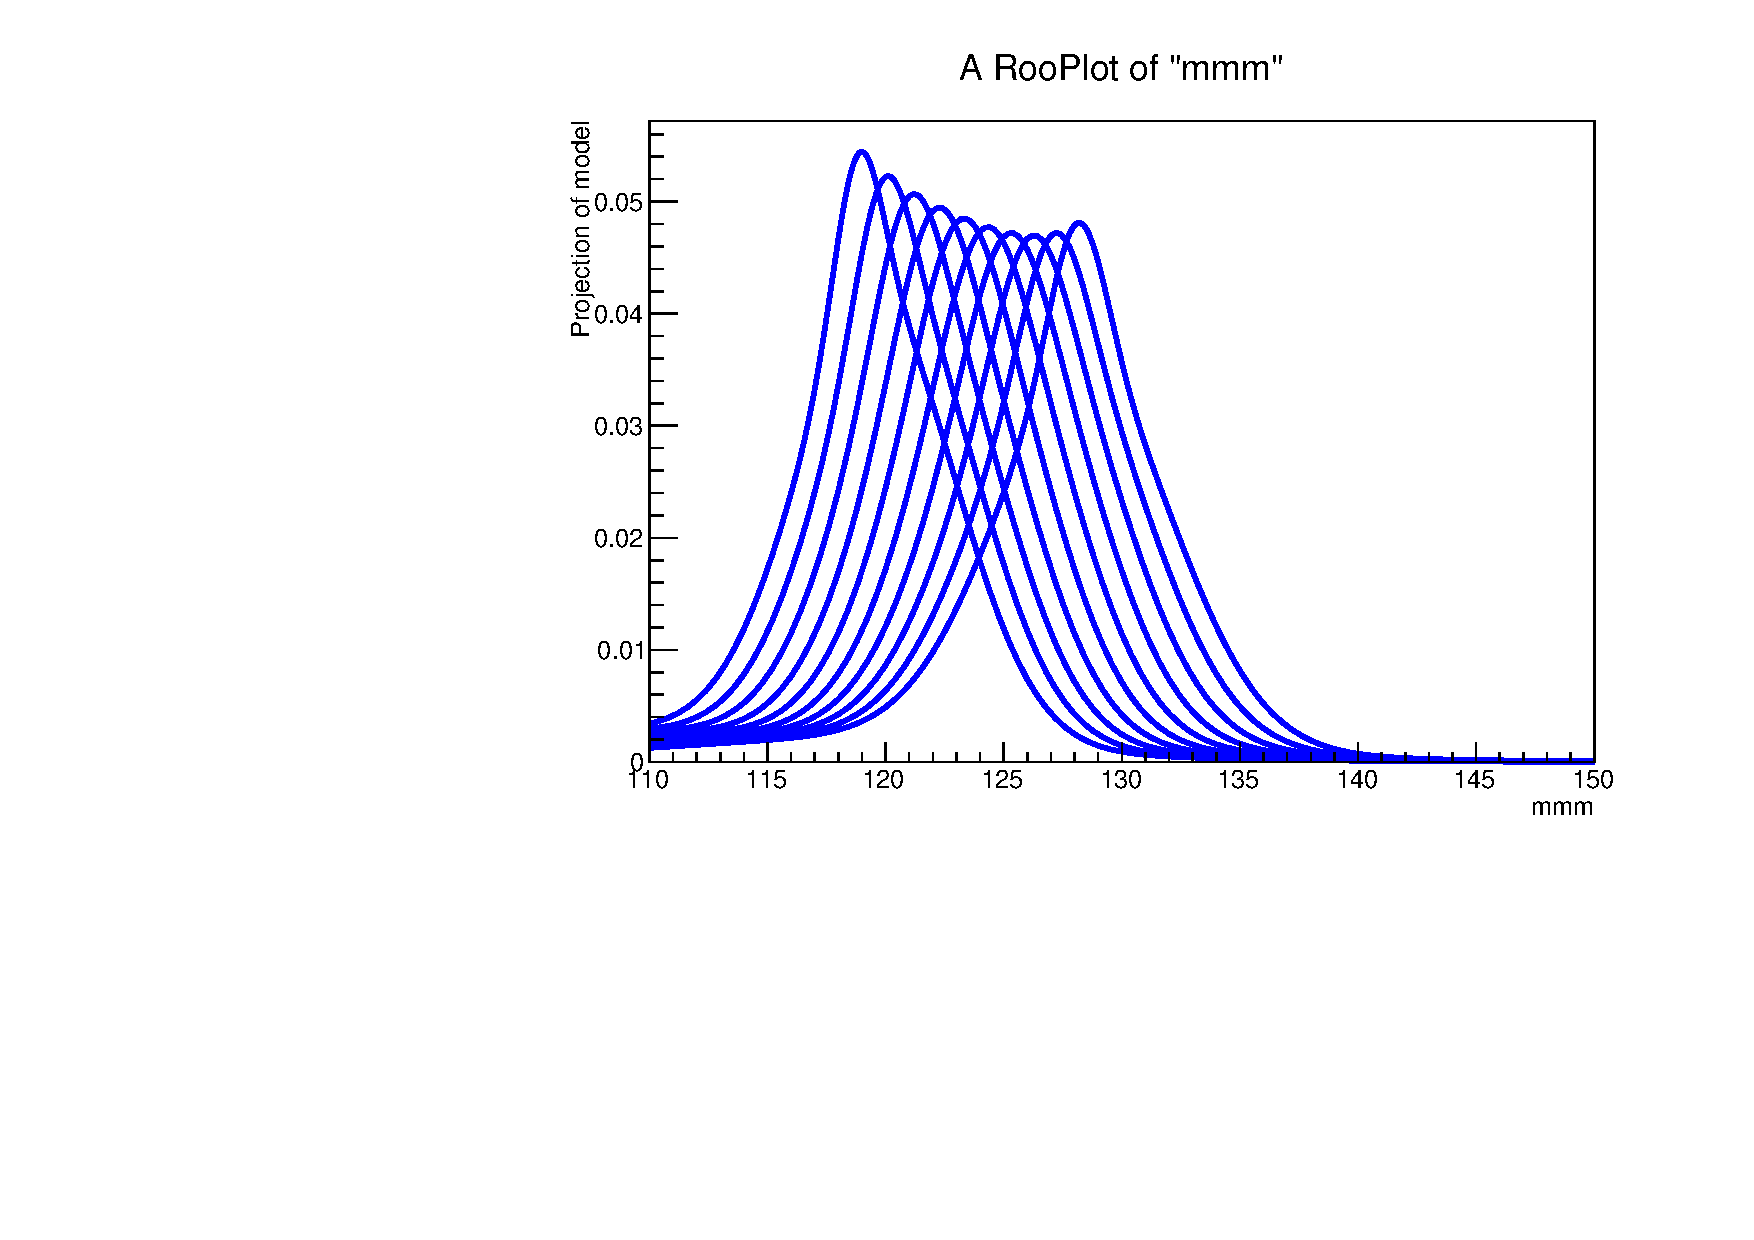
\includegraphics[width=0.49\linewidth]{figures/signal_model/AppendixBdt/interpolation_VBF_cat2.pdf}
  \caption{Signal Model Interpolation. Gluon Fusion (left column) and Vector Boson Fusion (right column). ''c0'' (top row), ''c1'' (middle row) and ''c2'' (bottom row)}
  \label{fig:higgs_signalmodel_gluvbfc0c2}
\end{figure}
\begin{figure}[hbp]
  \centering
  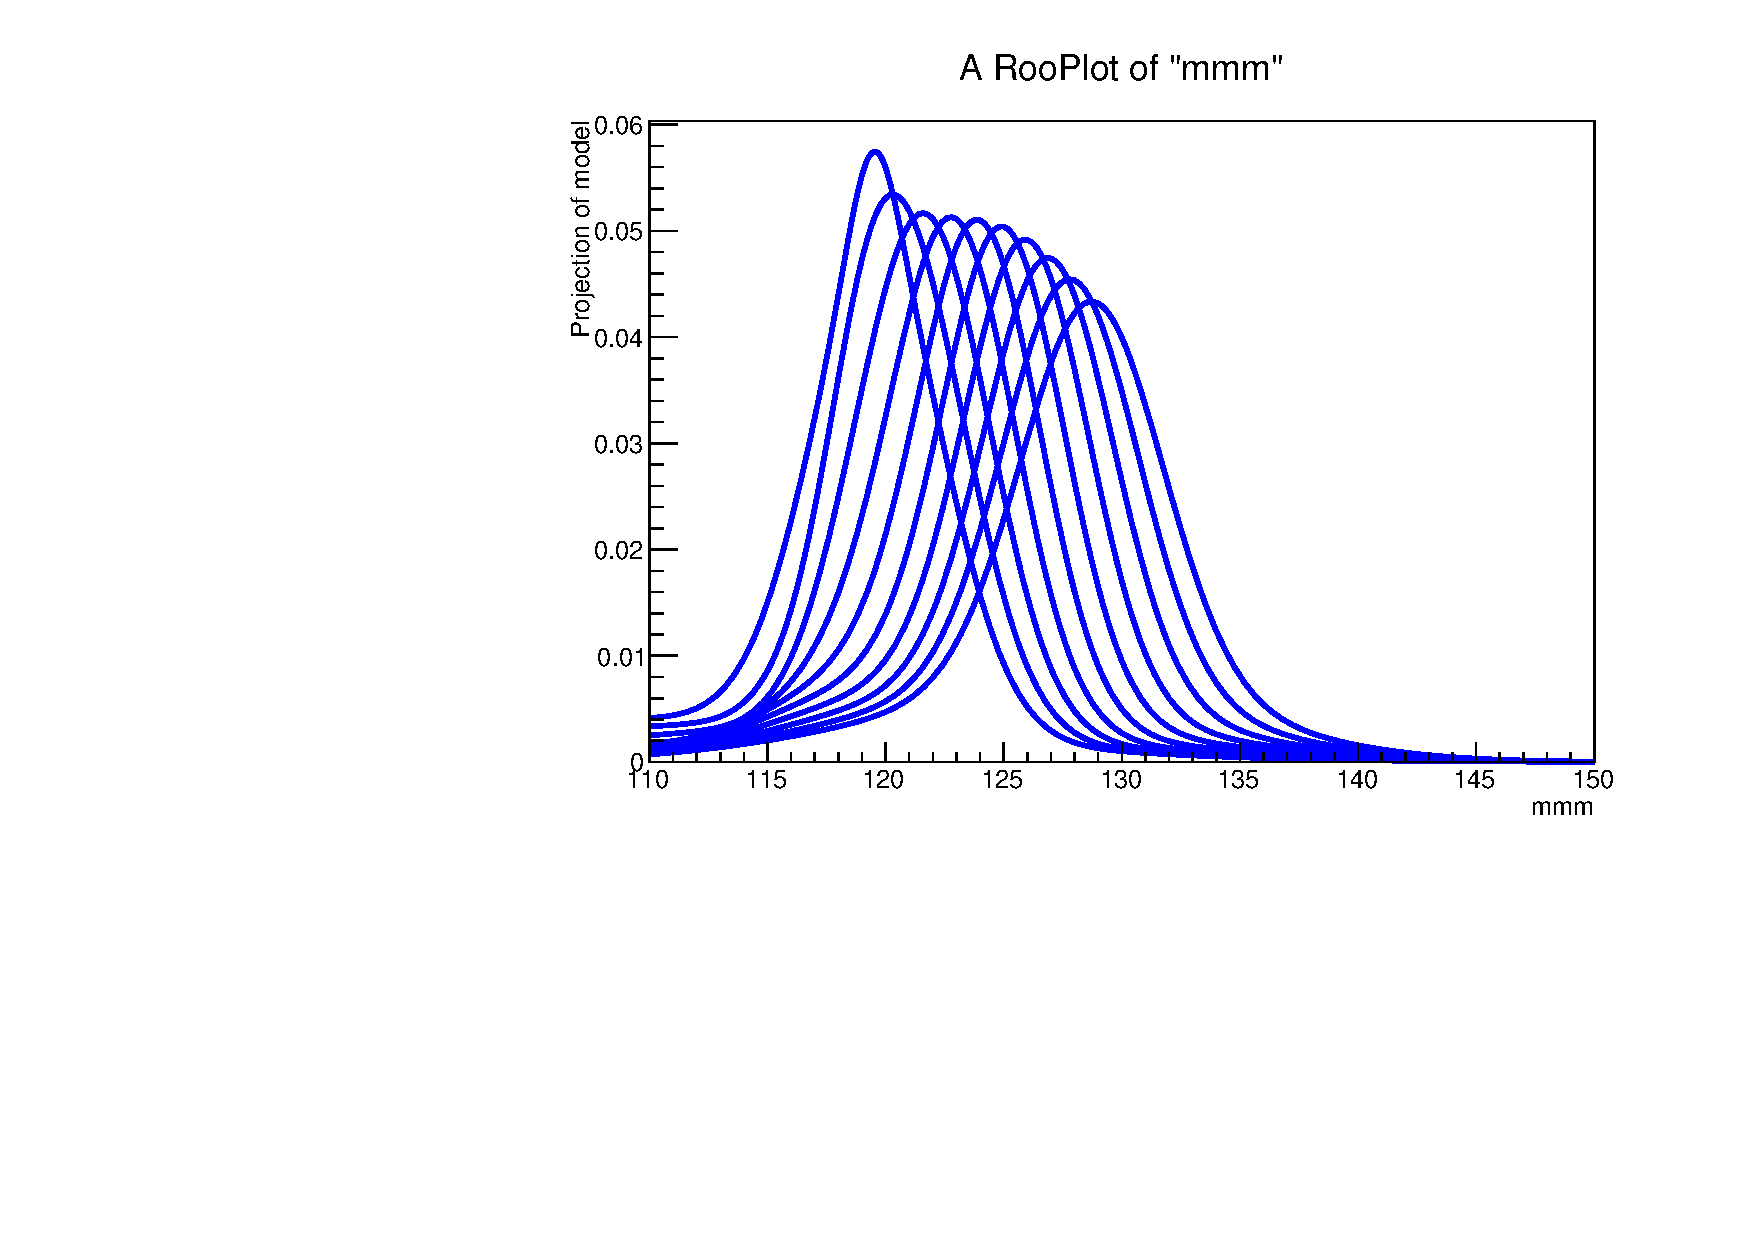
\includegraphics[width=0.49\linewidth]{figures/signal_model/AppendixBdt/interpolation_GluGlu_cat3.pdf}
  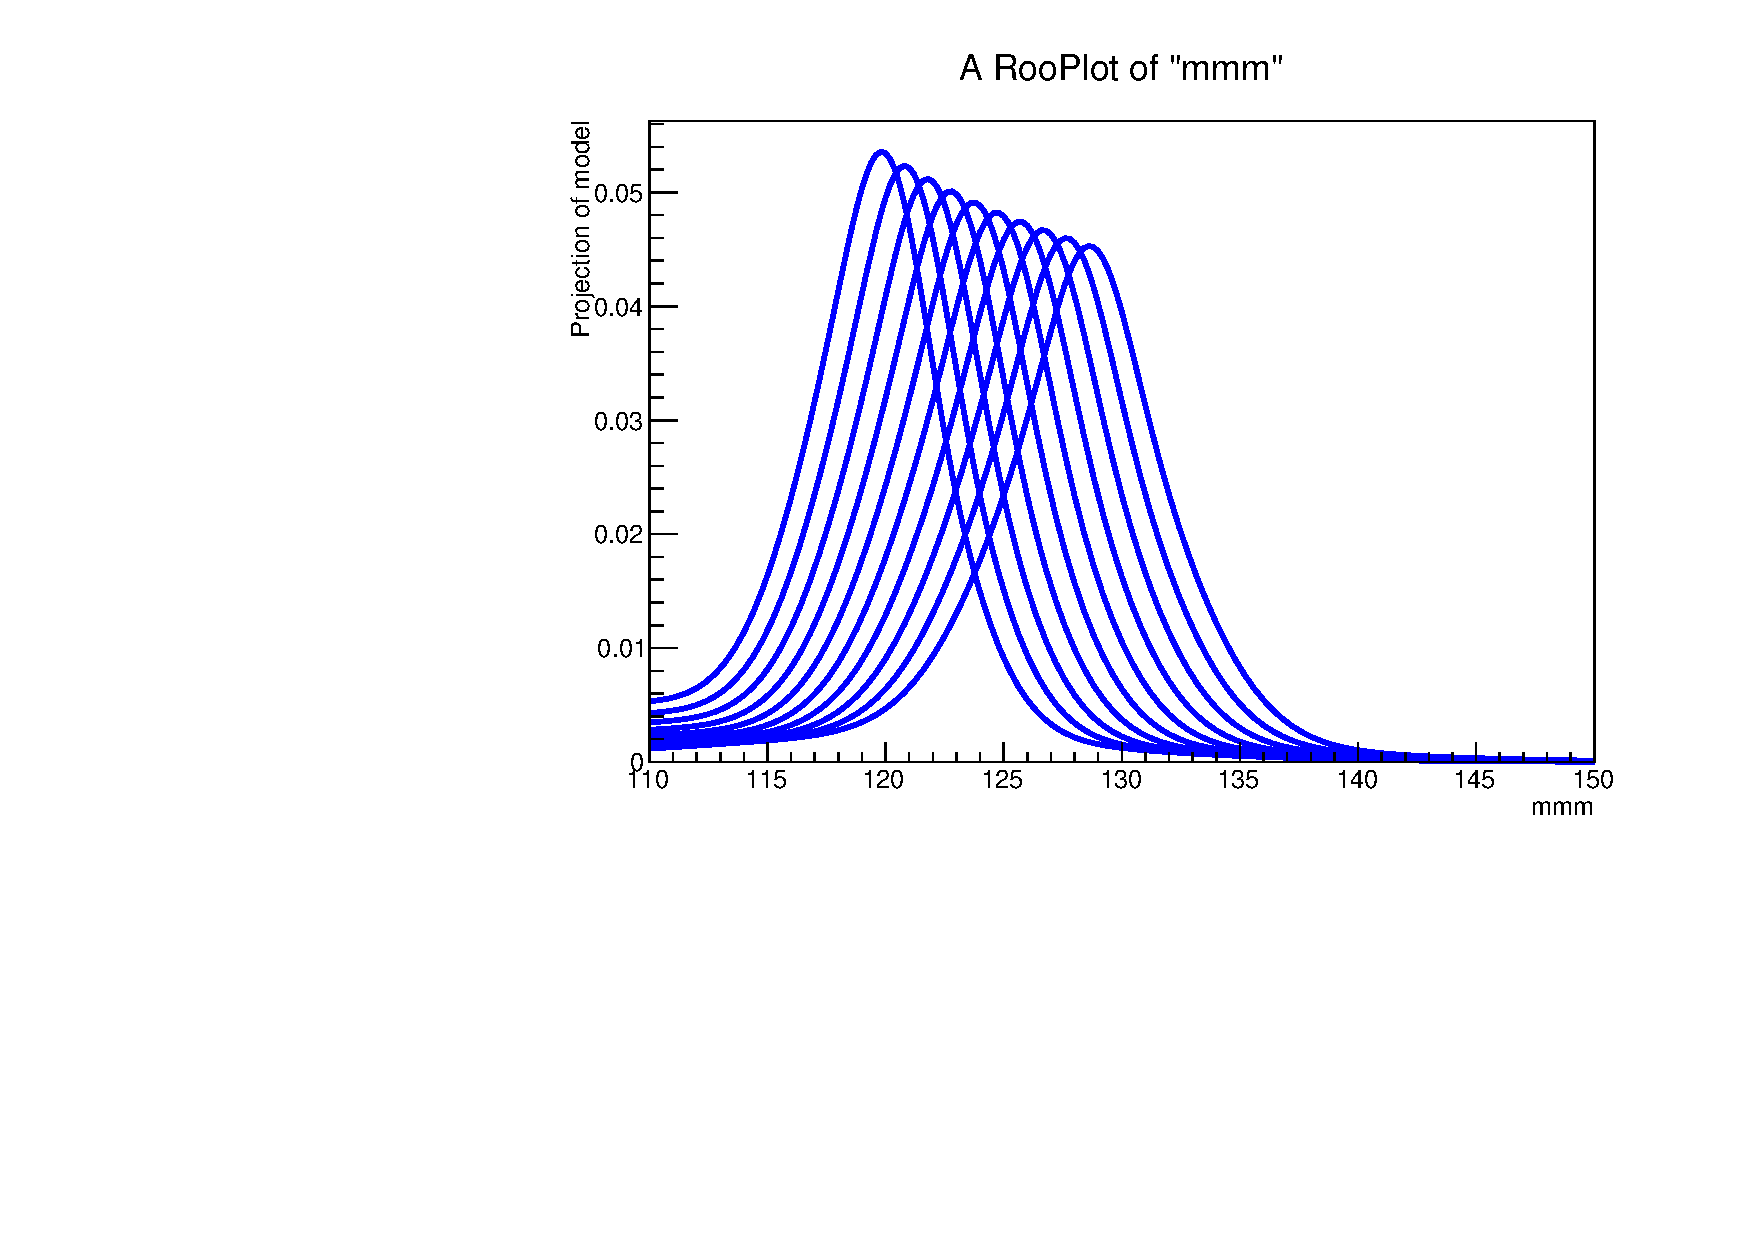
\includegraphics[width=0.49\linewidth]{figures/signal_model/AppendixBdt/interpolation_VBF_cat3.pdf}\\
  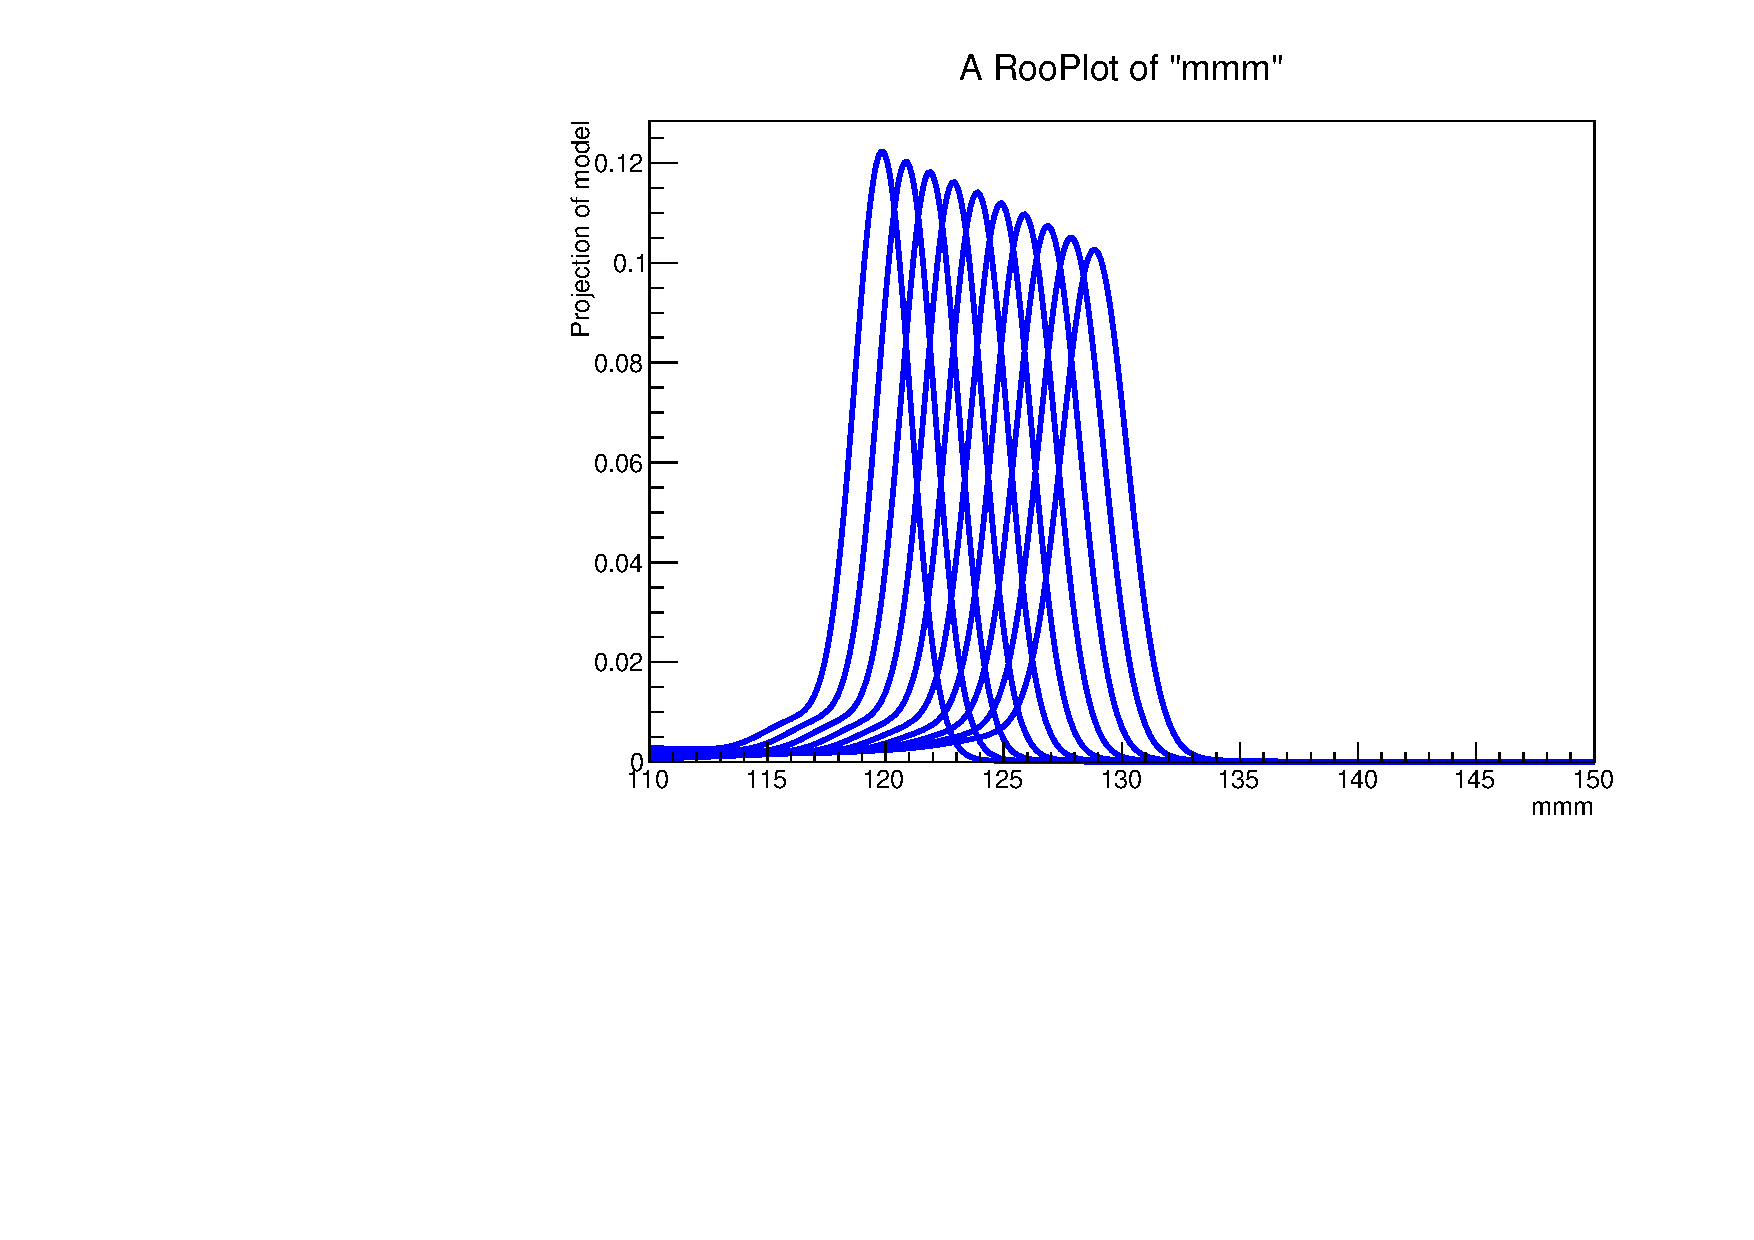
\includegraphics[width=0.49\linewidth]{figures/signal_model/AppendixBdt/interpolation_GluGlu_cat4.pdf}
  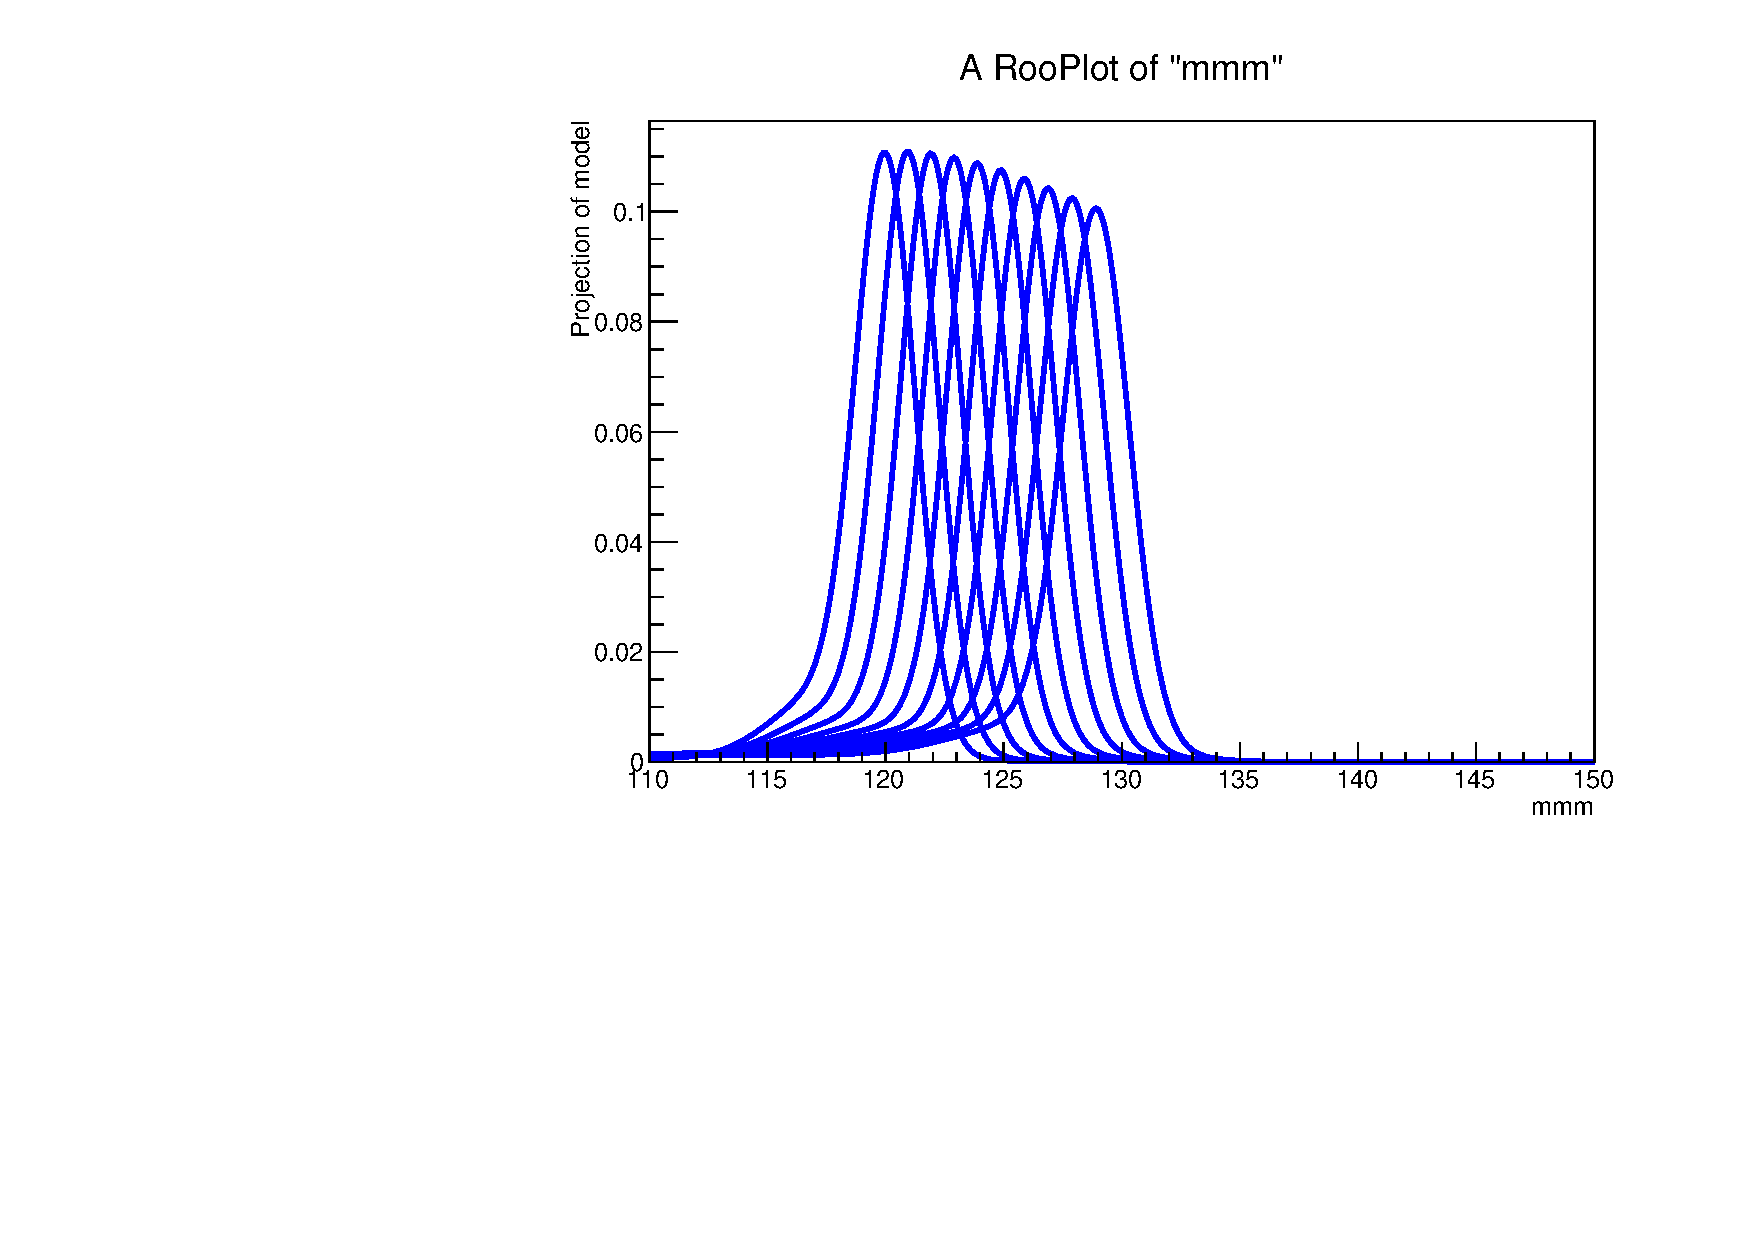
\includegraphics[width=0.49\linewidth]{figures/signal_model/AppendixBdt/interpolation_VBF_cat4.pdf}\\
  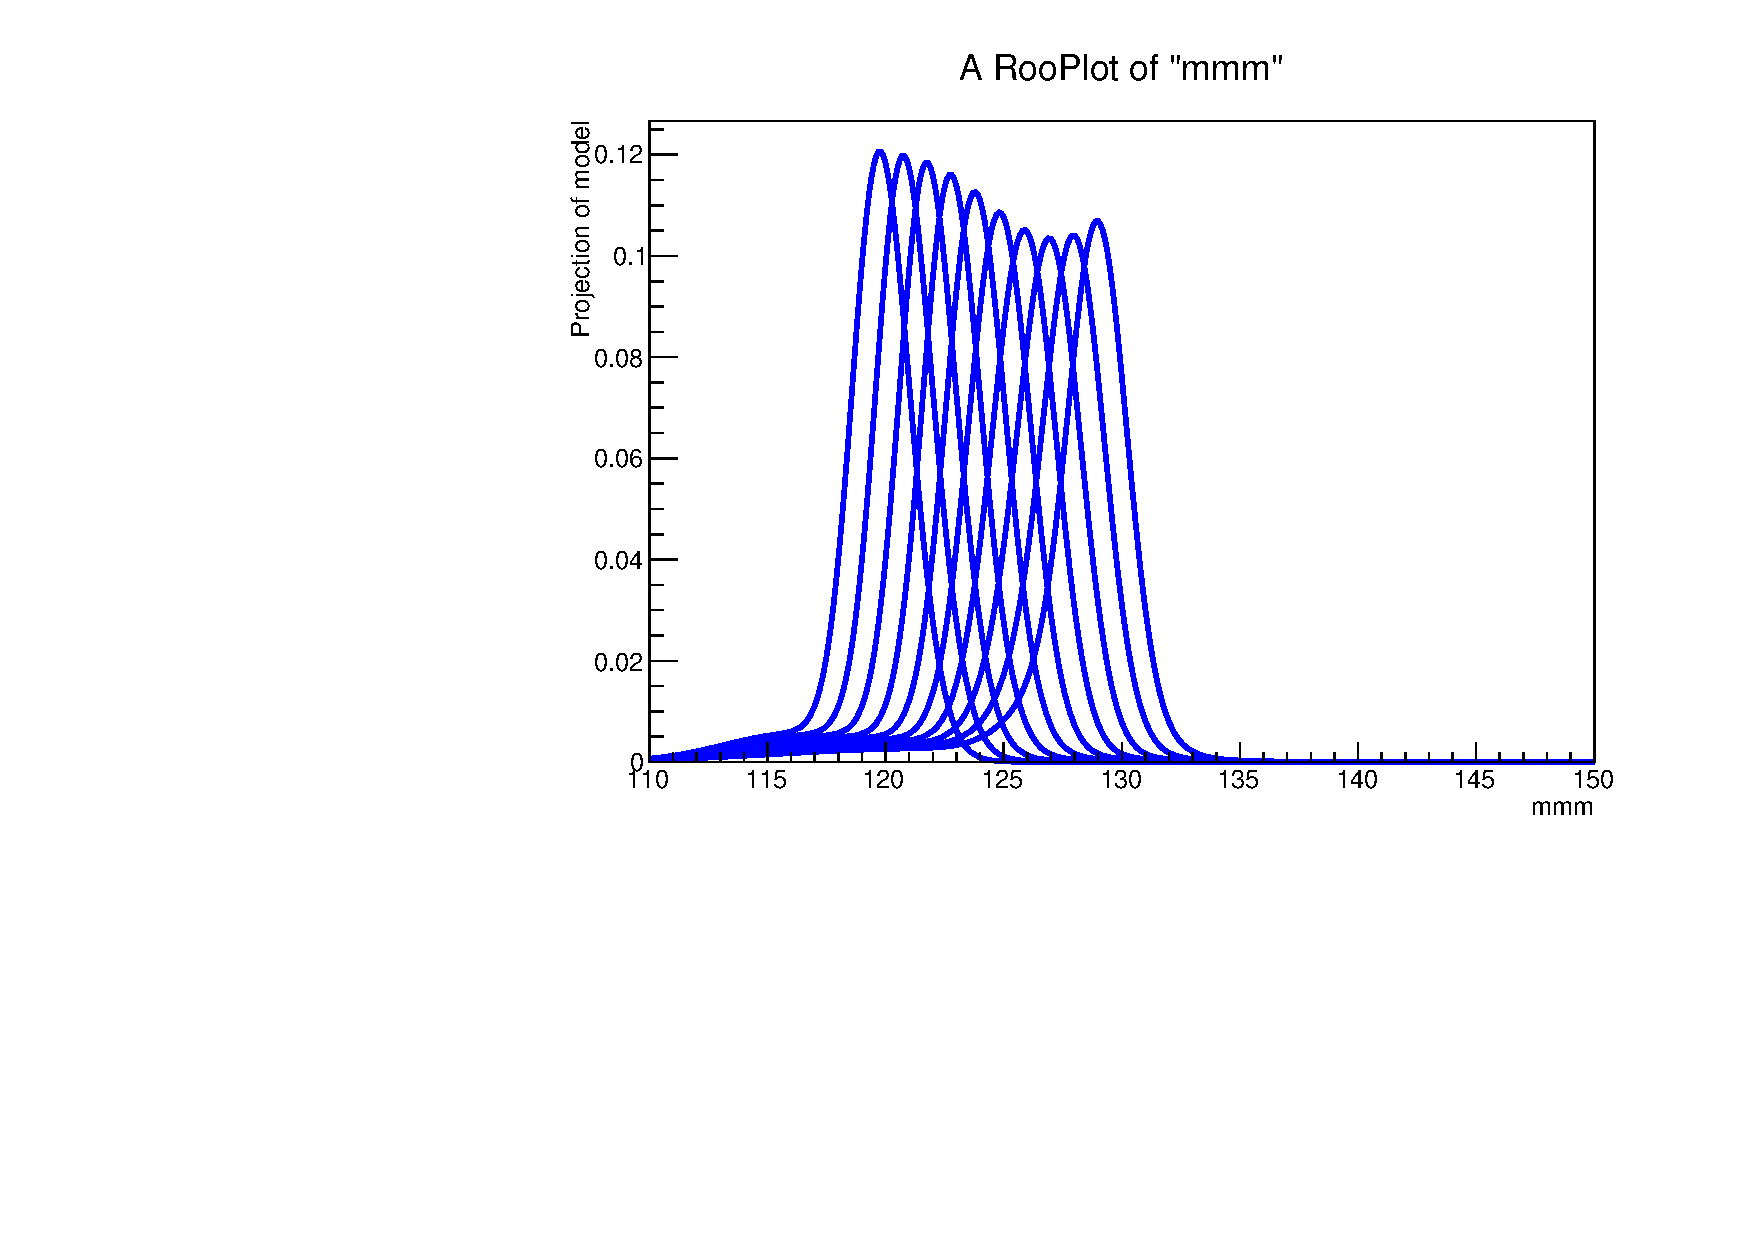
\includegraphics[width=0.49\linewidth]{figures/signal_model/AppendixBdt/interpolation_GluGlu_cat5.pdf}
  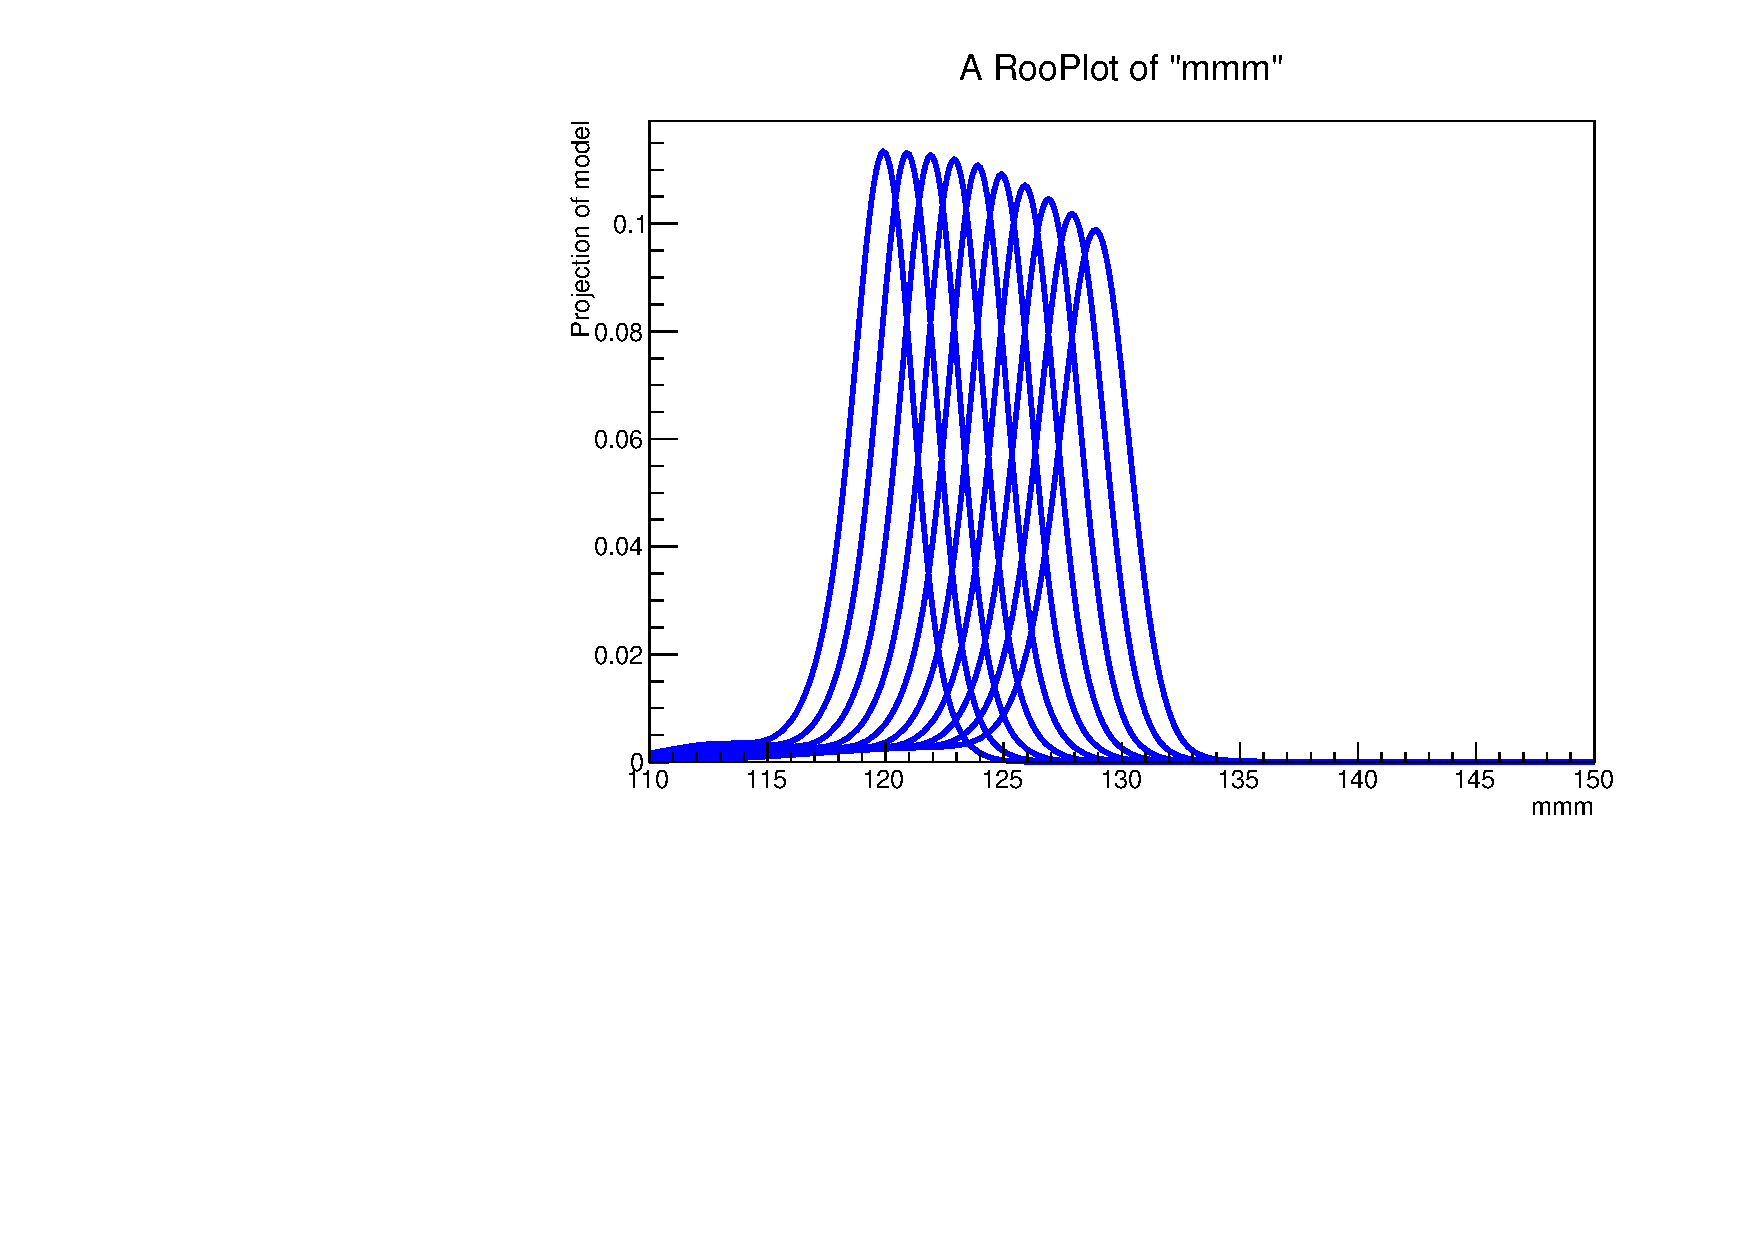
\includegraphics[width=0.49\linewidth]{figures/signal_model/AppendixBdt/interpolation_VBF_cat5.pdf}
  \caption{Signal Model Interpolation. Gluon Fusion (left column) and Vector Boson Fusion (right column). ''c3'' (top row), ''c4'' (middle row) and ''c5'' (bottom row)}
  \label{fig:higgs_signalmodel_gluvbfc3c5}
\end{figure}
\begin{figure}[hbp]
  \centering
  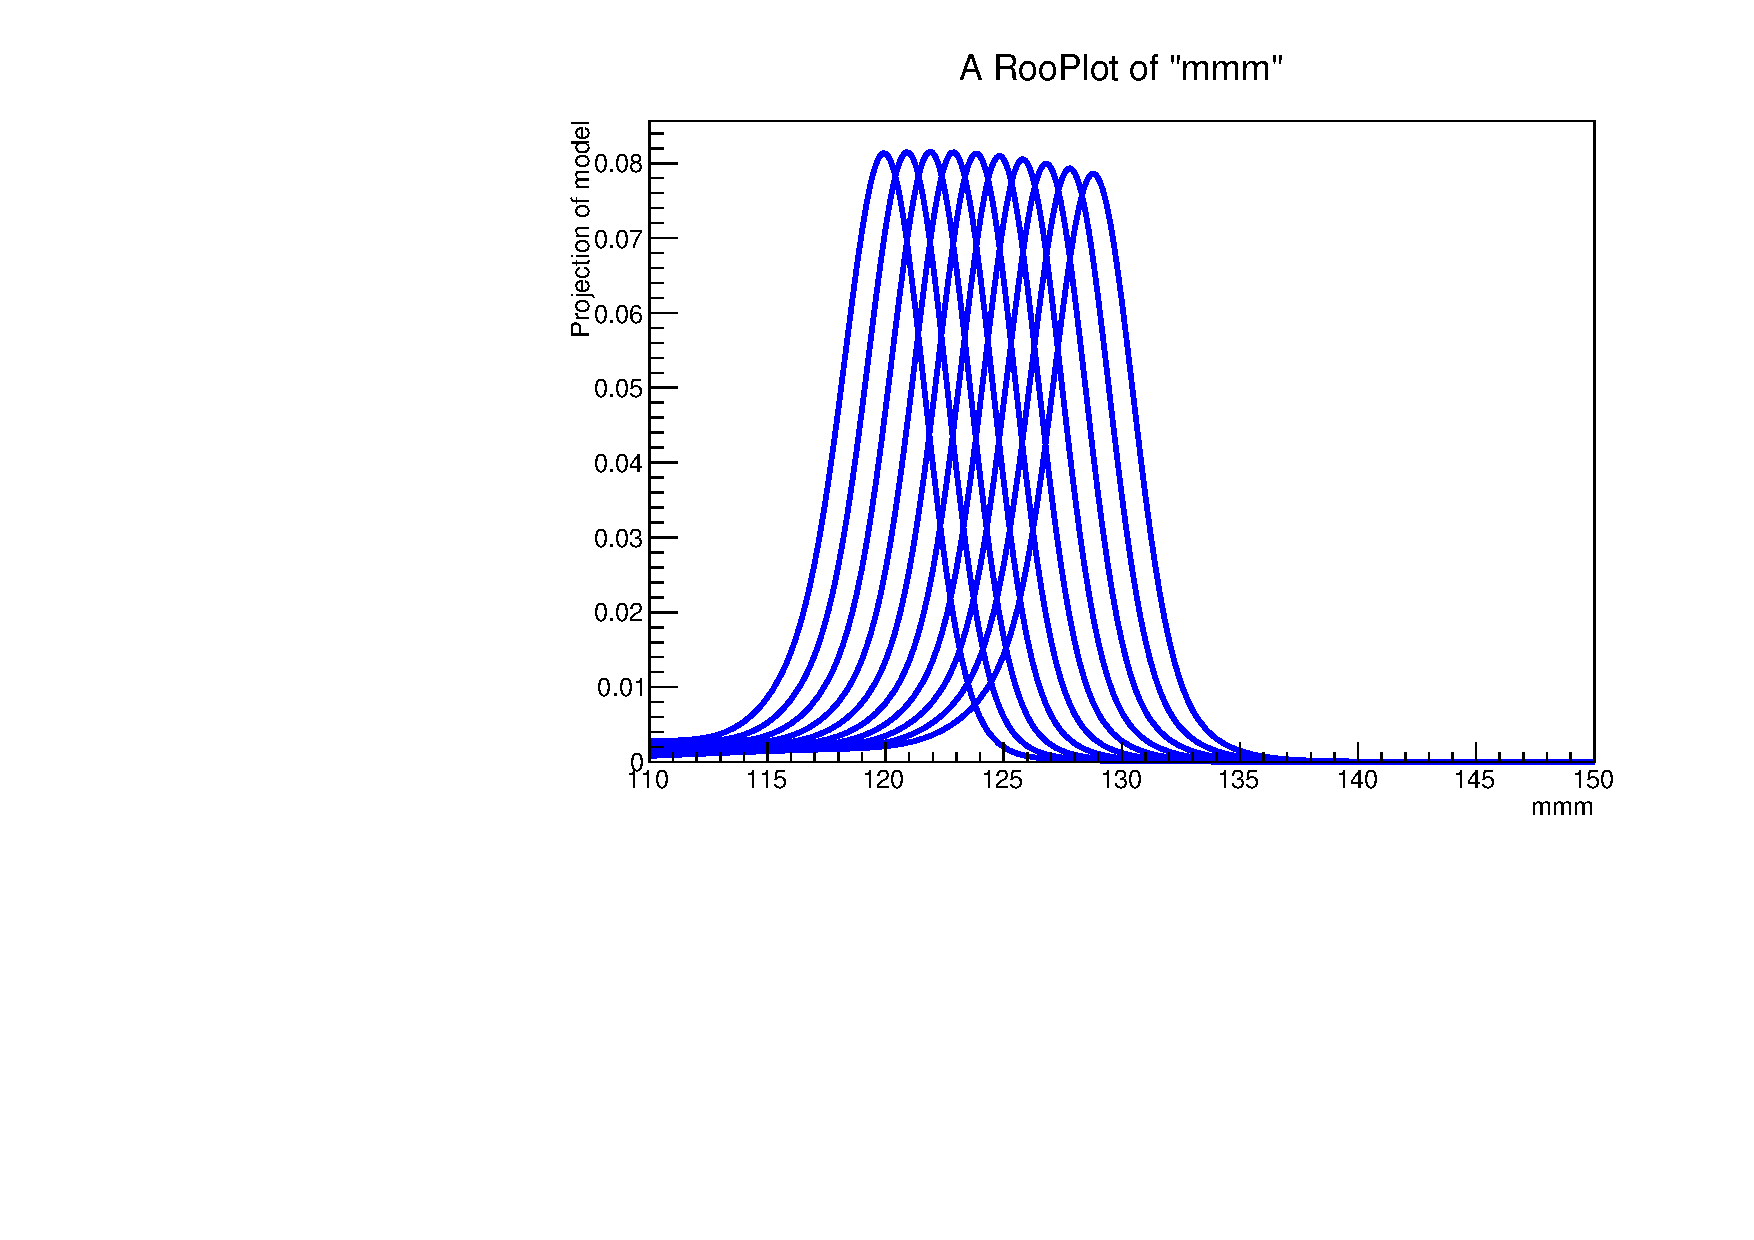
\includegraphics[width=0.49\linewidth]{figures/signal_model/AppendixBdt/interpolation_GluGlu_cat6.pdf}
  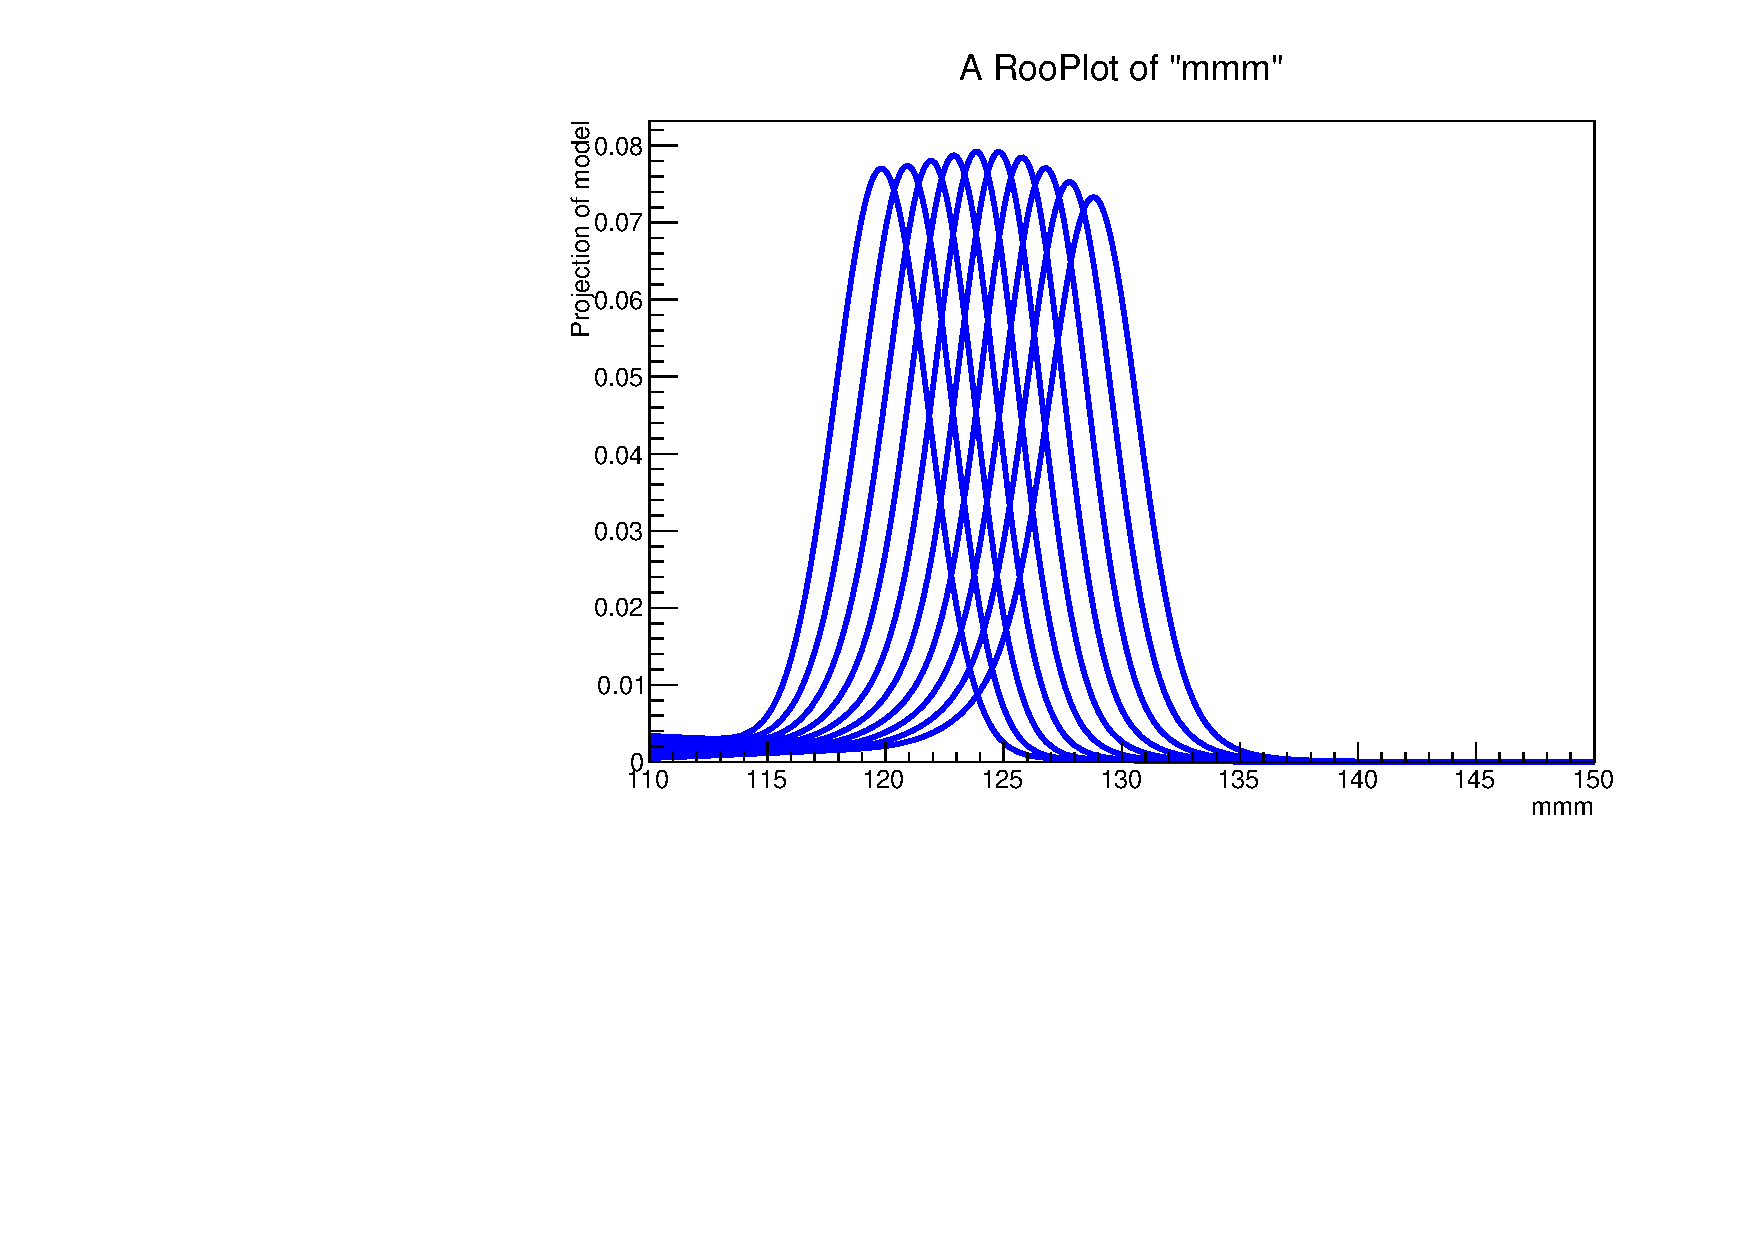
\includegraphics[width=0.49\linewidth]{figures/signal_model/AppendixBdt/interpolation_VBF_cat6.pdf}\\
  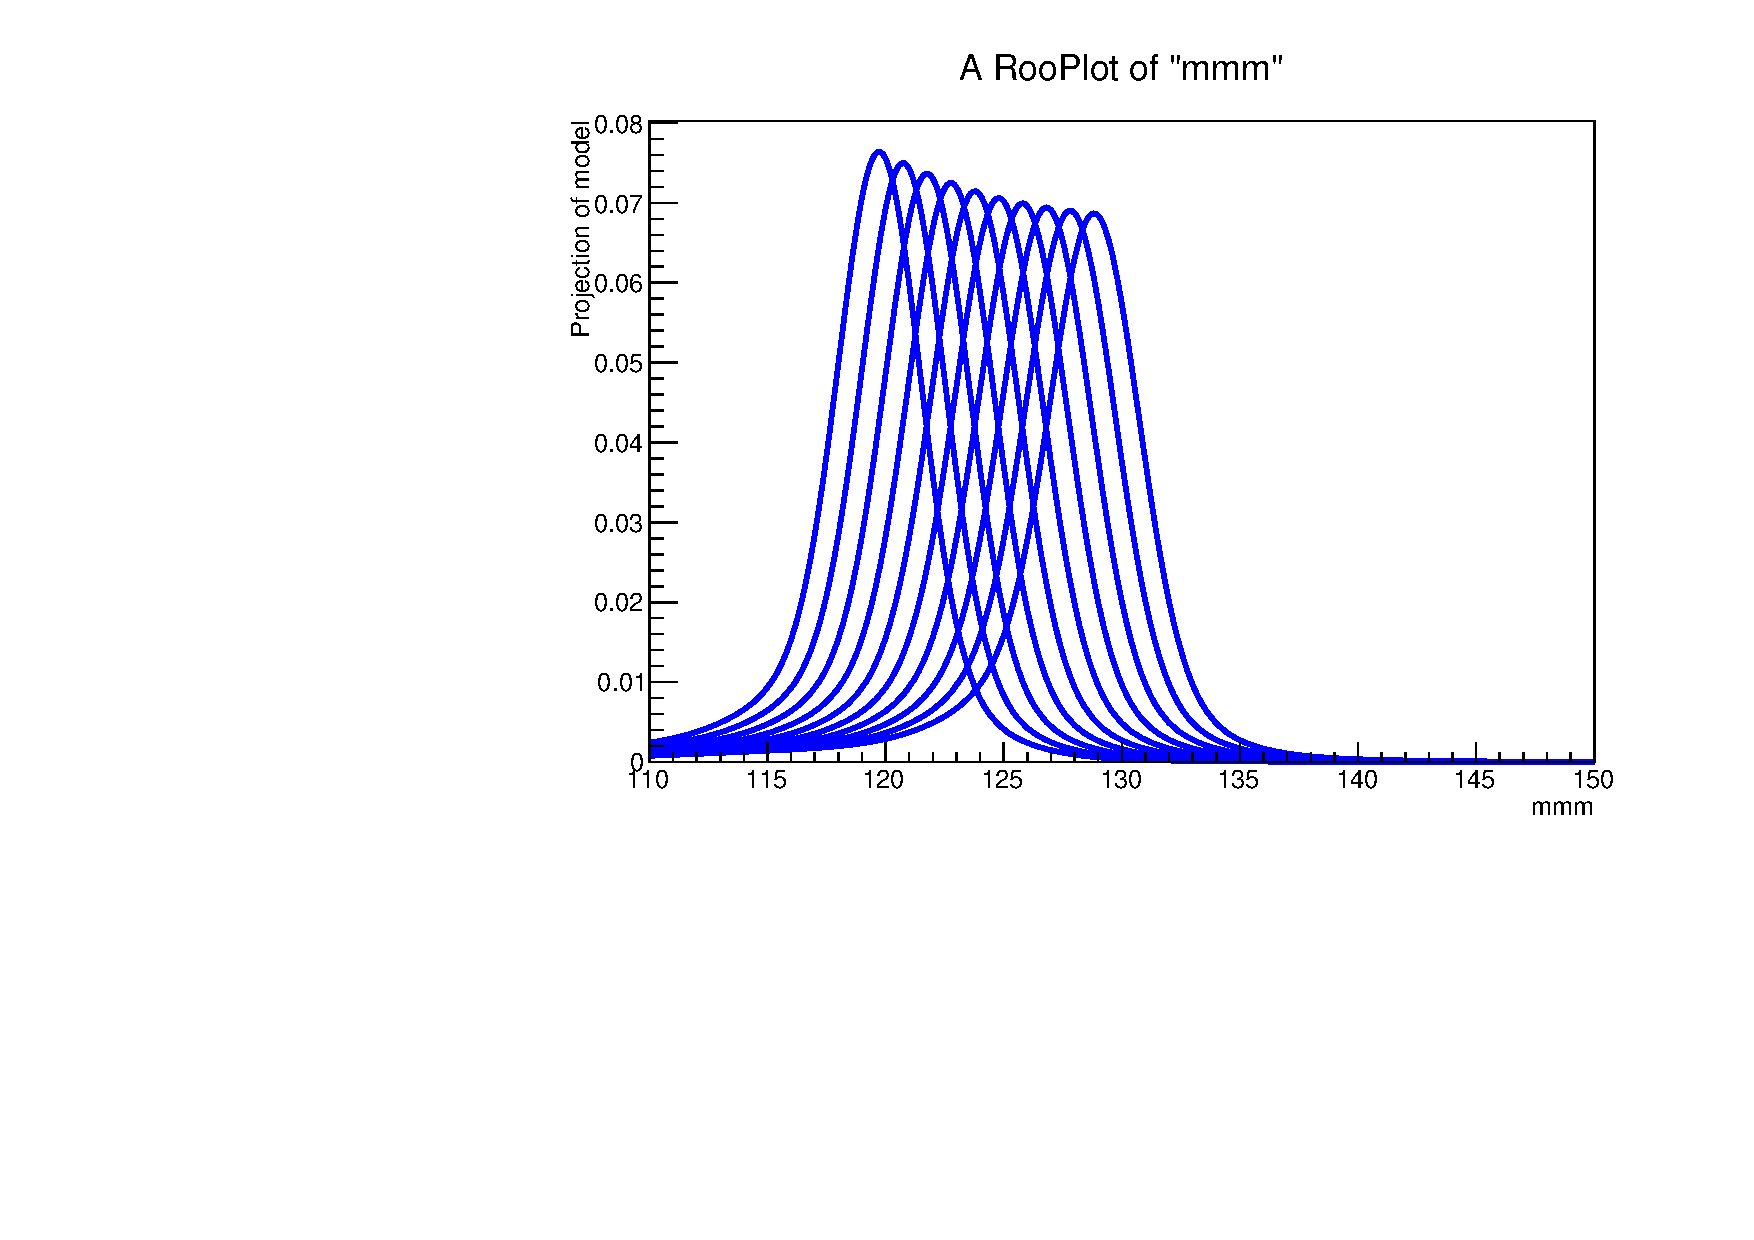
\includegraphics[width=0.49\linewidth]{figures/signal_model/AppendixBdt/interpolation_GluGlu_cat7.pdf}
  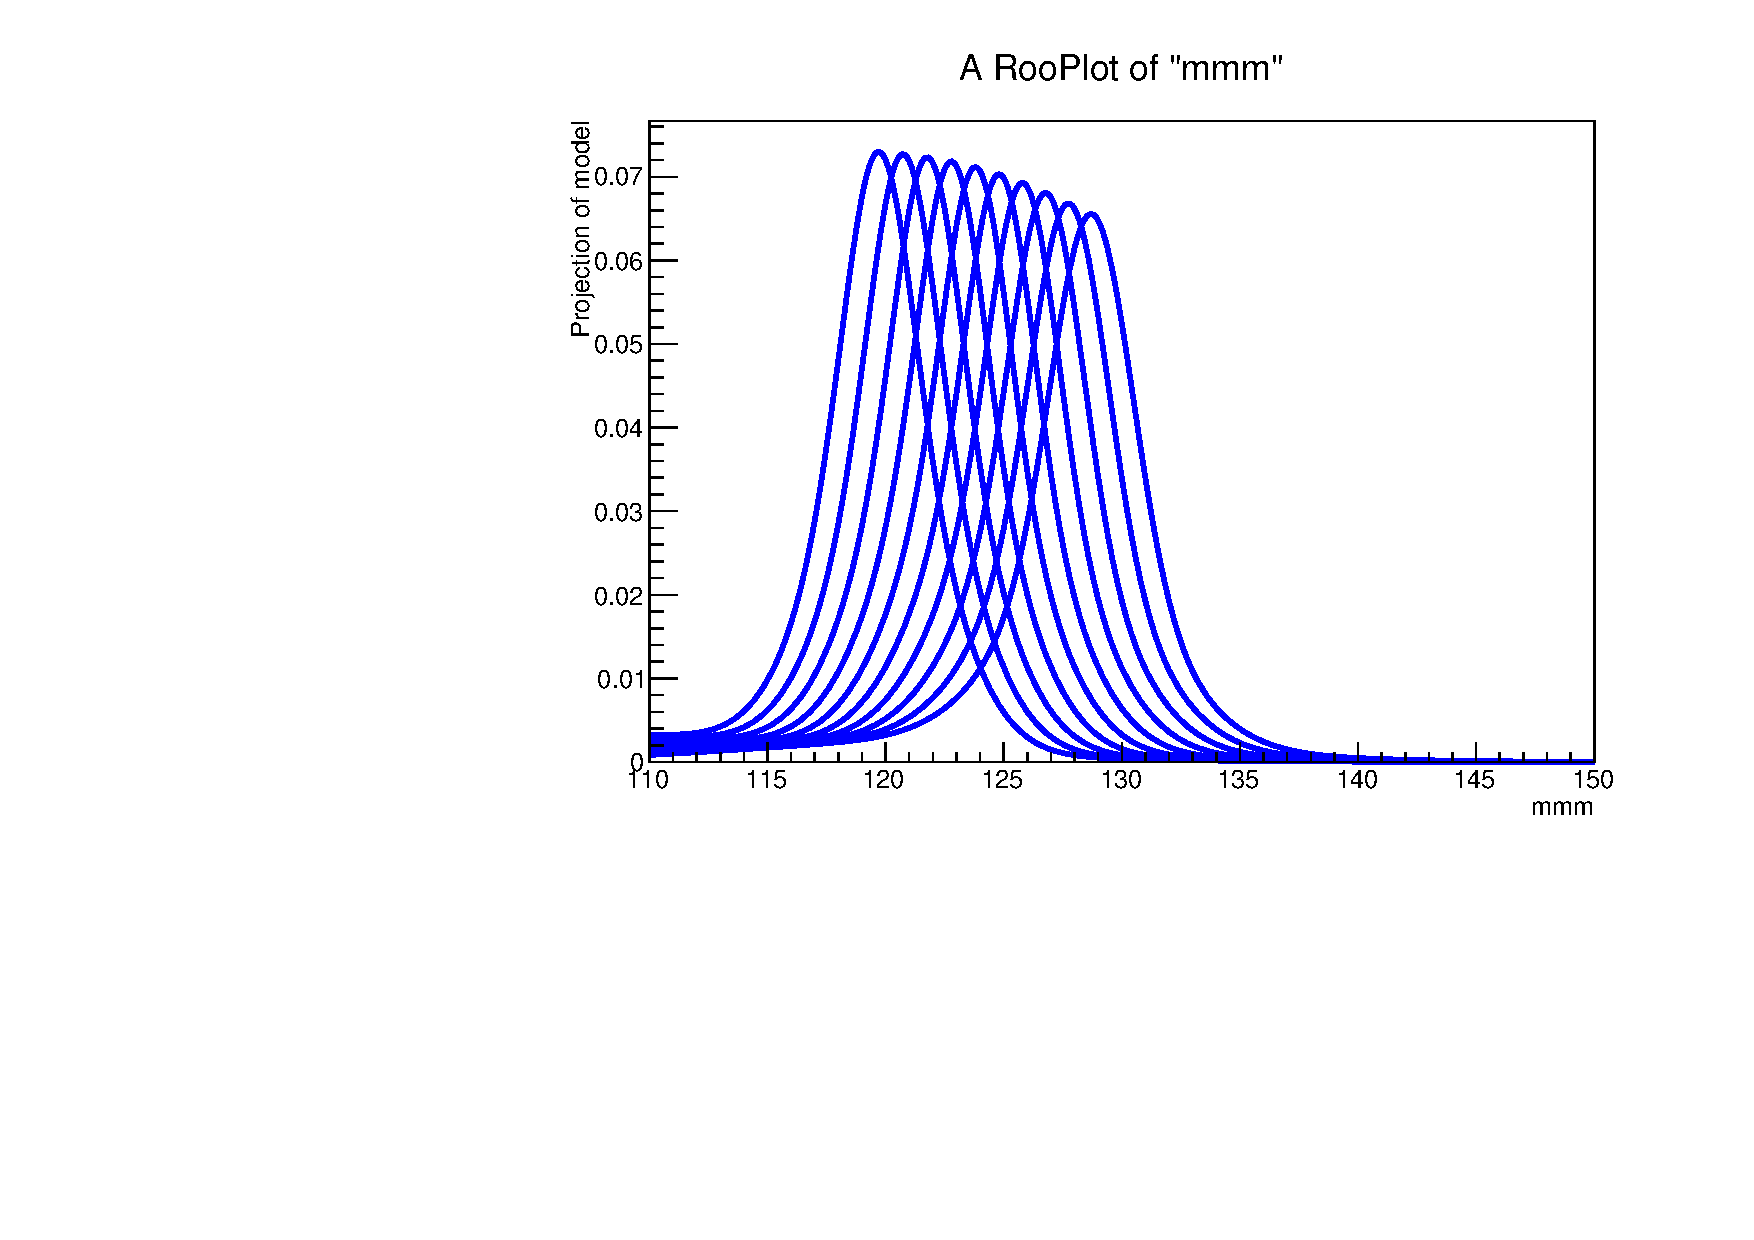
\includegraphics[width=0.49\linewidth]{figures/signal_model/AppendixBdt/interpolation_VBF_cat7.pdf}\\
  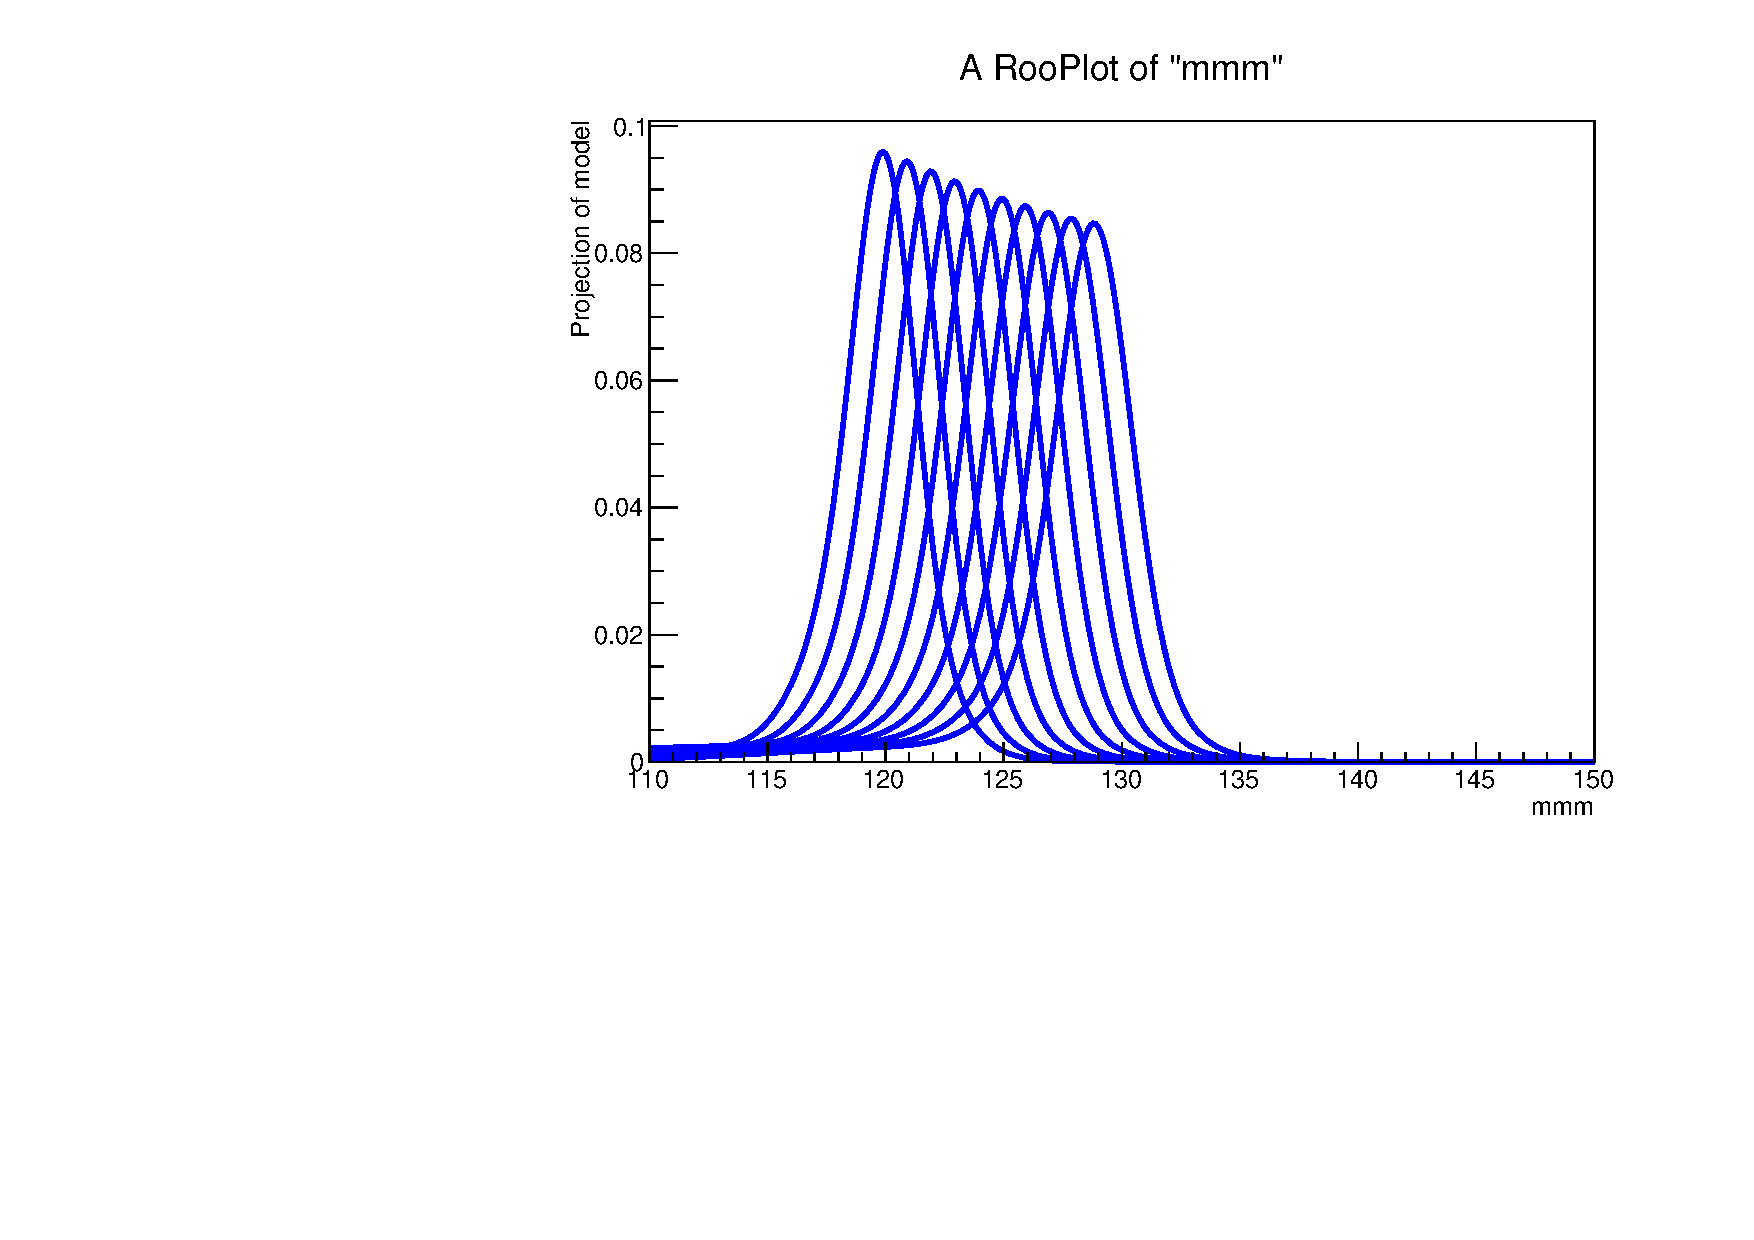
\includegraphics[width=0.49\linewidth]{figures/signal_model/AppendixBdt/interpolation_GluGlu_cat8.pdf}
  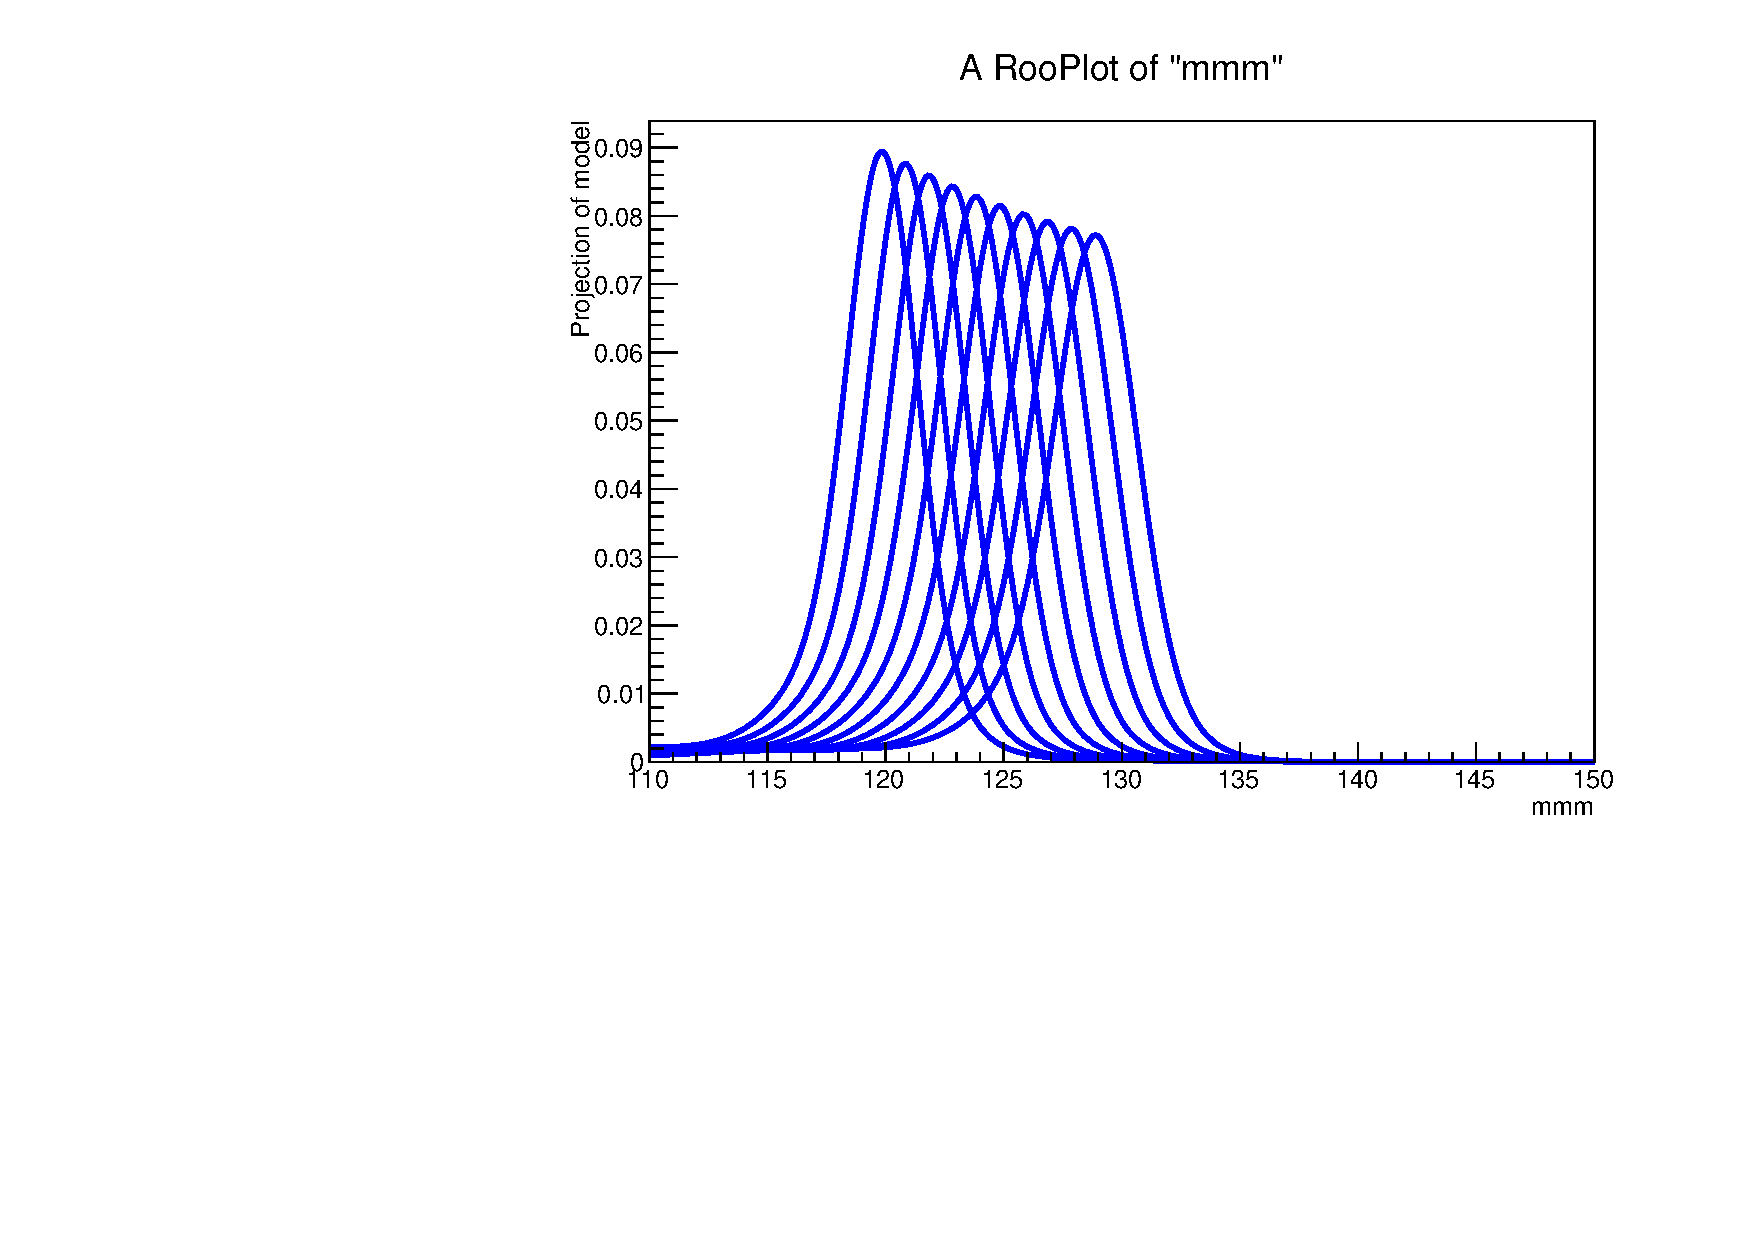
\includegraphics[width=0.49\linewidth]{figures/signal_model/AppendixBdt/interpolation_VBF_cat8.pdf}
  \caption{Signal Model Interpolation. Gluon Fusion (left column) and Vector Boson Fusion (right column). ''c6'' (top row), ''c7'' (middle row) and ''c8'' (bottom row)}
  \label{fig:higgs_signalmodel_gluvbfc6c8}
\end{figure}
\begin{figure}[hbp]
  \centering
  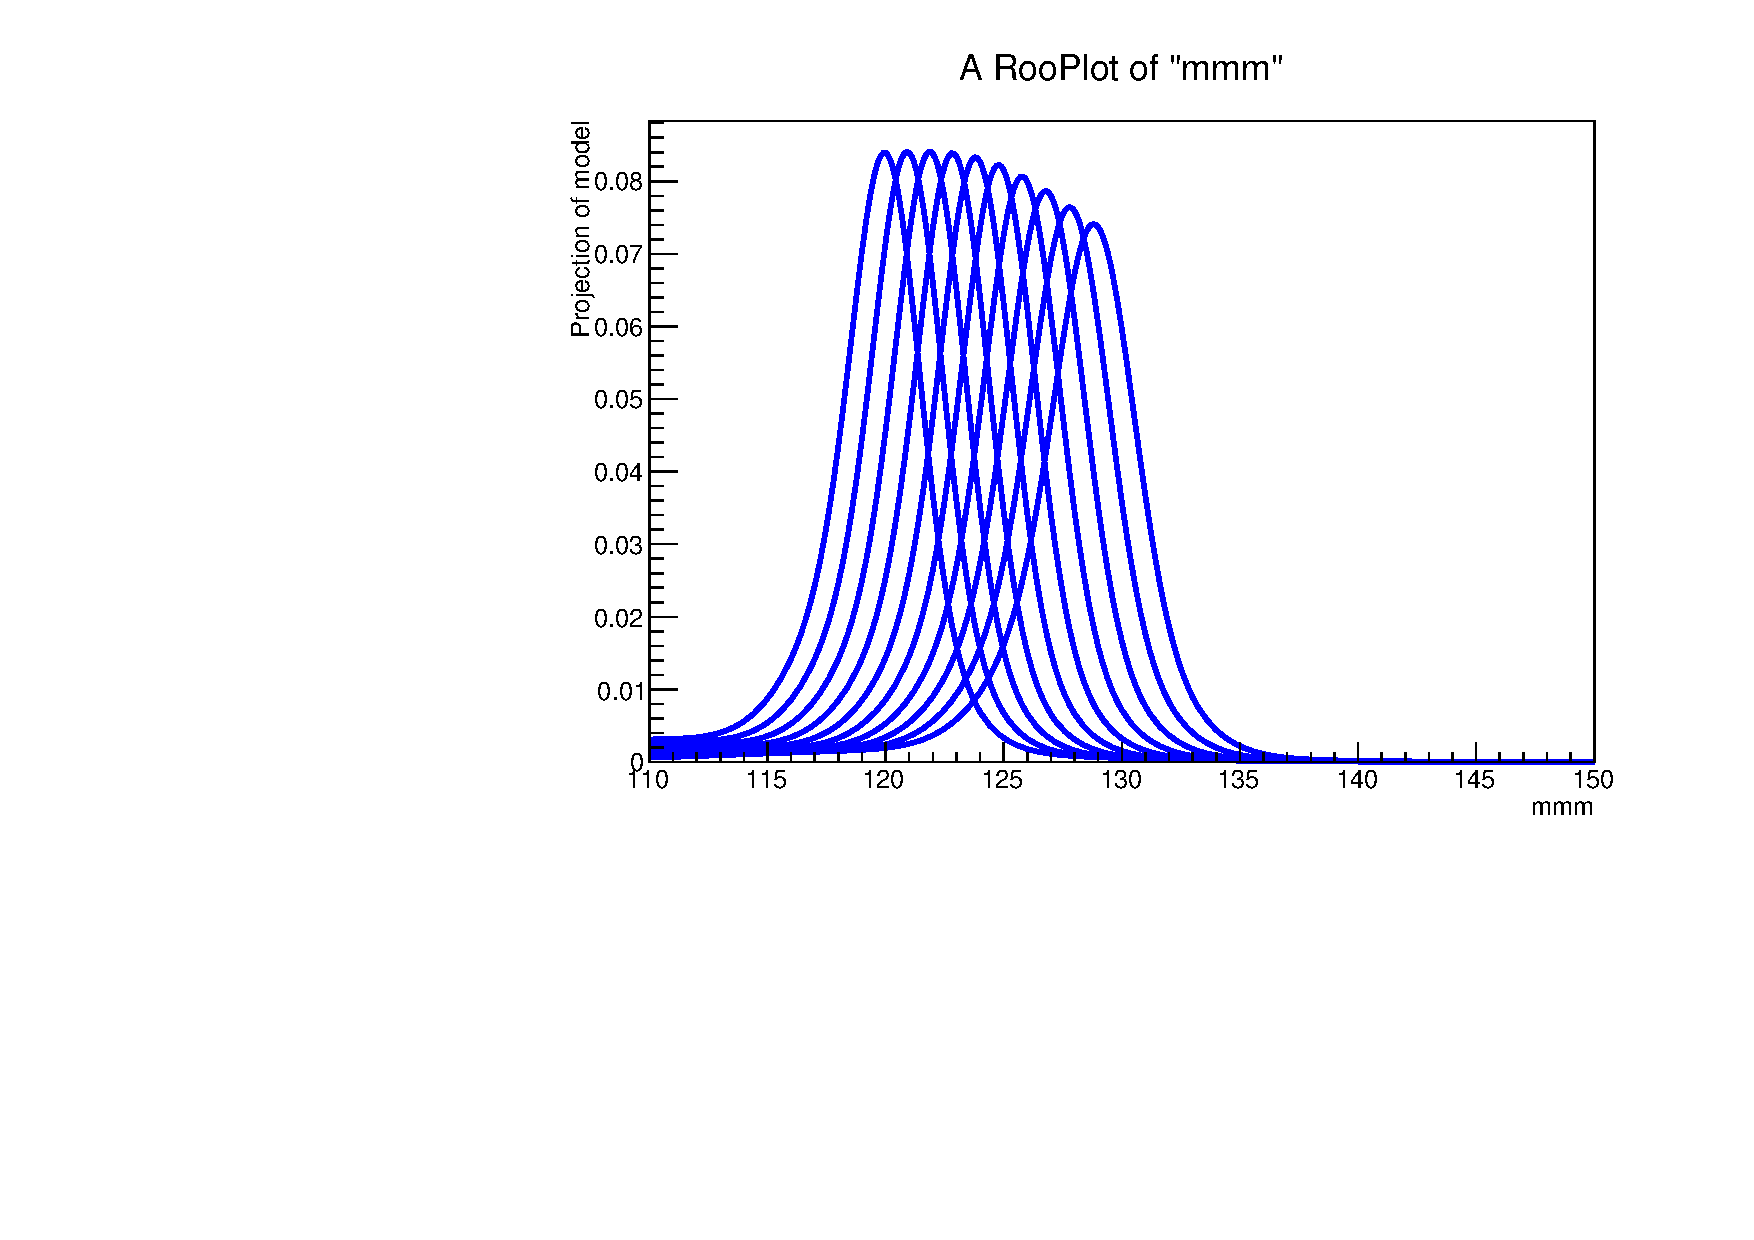
\includegraphics[width=0.49\linewidth]{figures/signal_model/AppendixBdt/interpolation_GluGlu_cat9.pdf}
  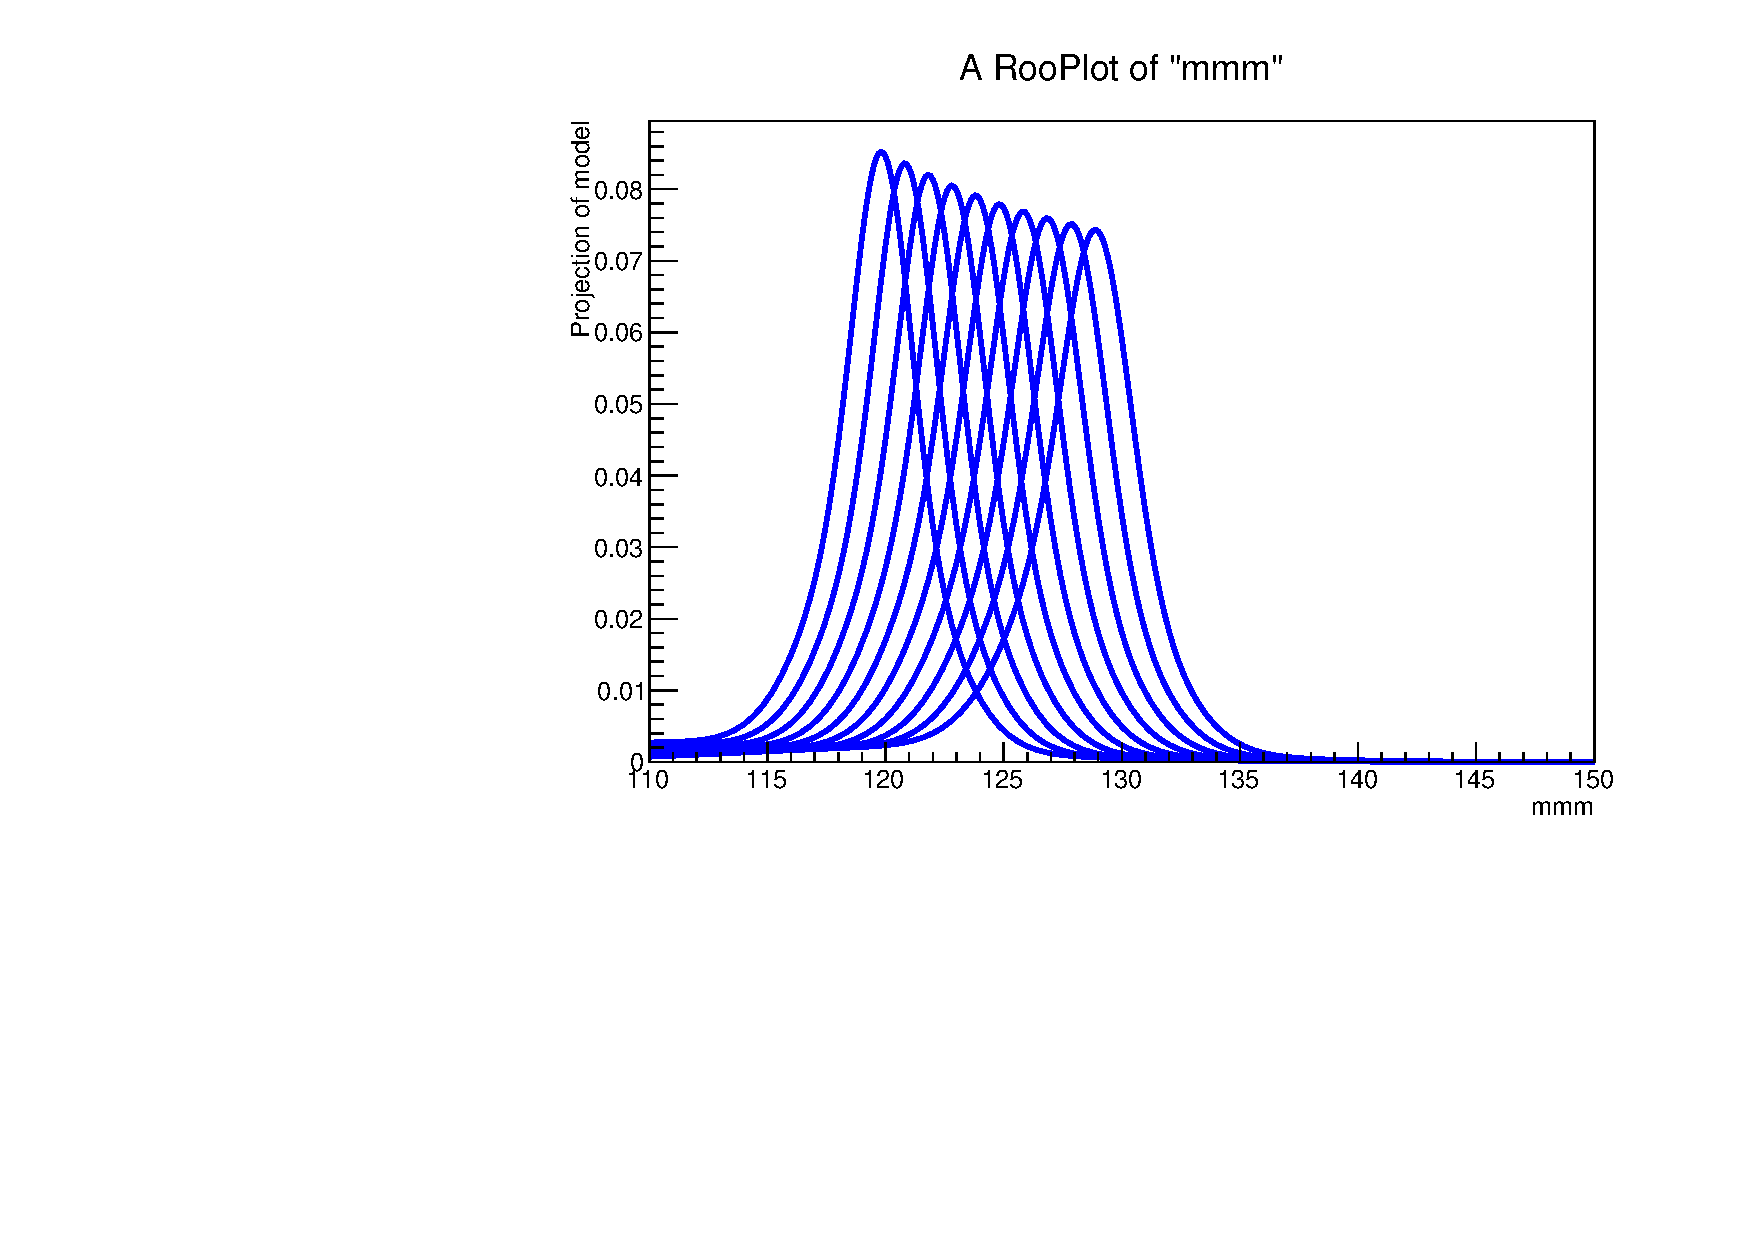
\includegraphics[width=0.49\linewidth]{figures/signal_model/AppendixBdt/interpolation_VBF_cat9.pdf}\\
  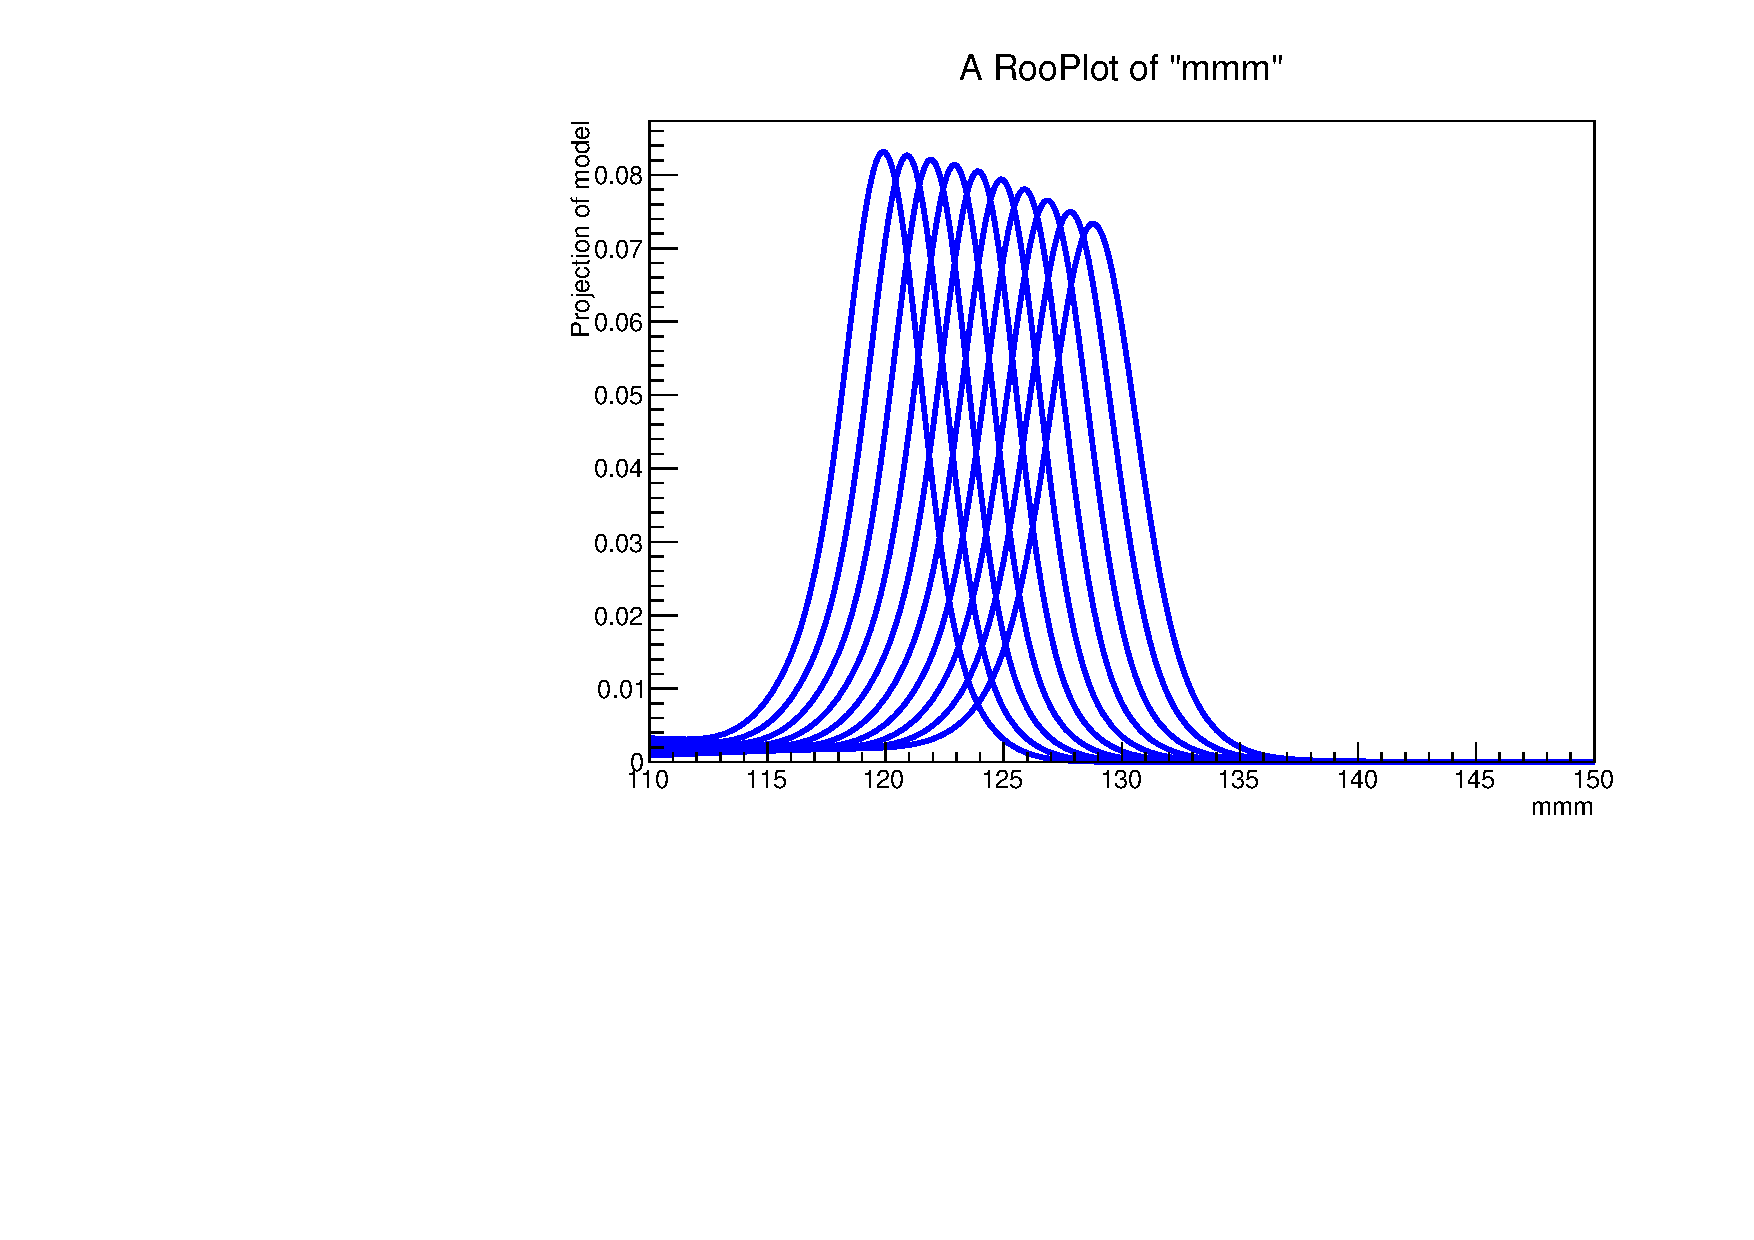
\includegraphics[width=0.49\linewidth]{figures/signal_model/AppendixBdt/interpolation_GluGlu_cat10.pdf}
  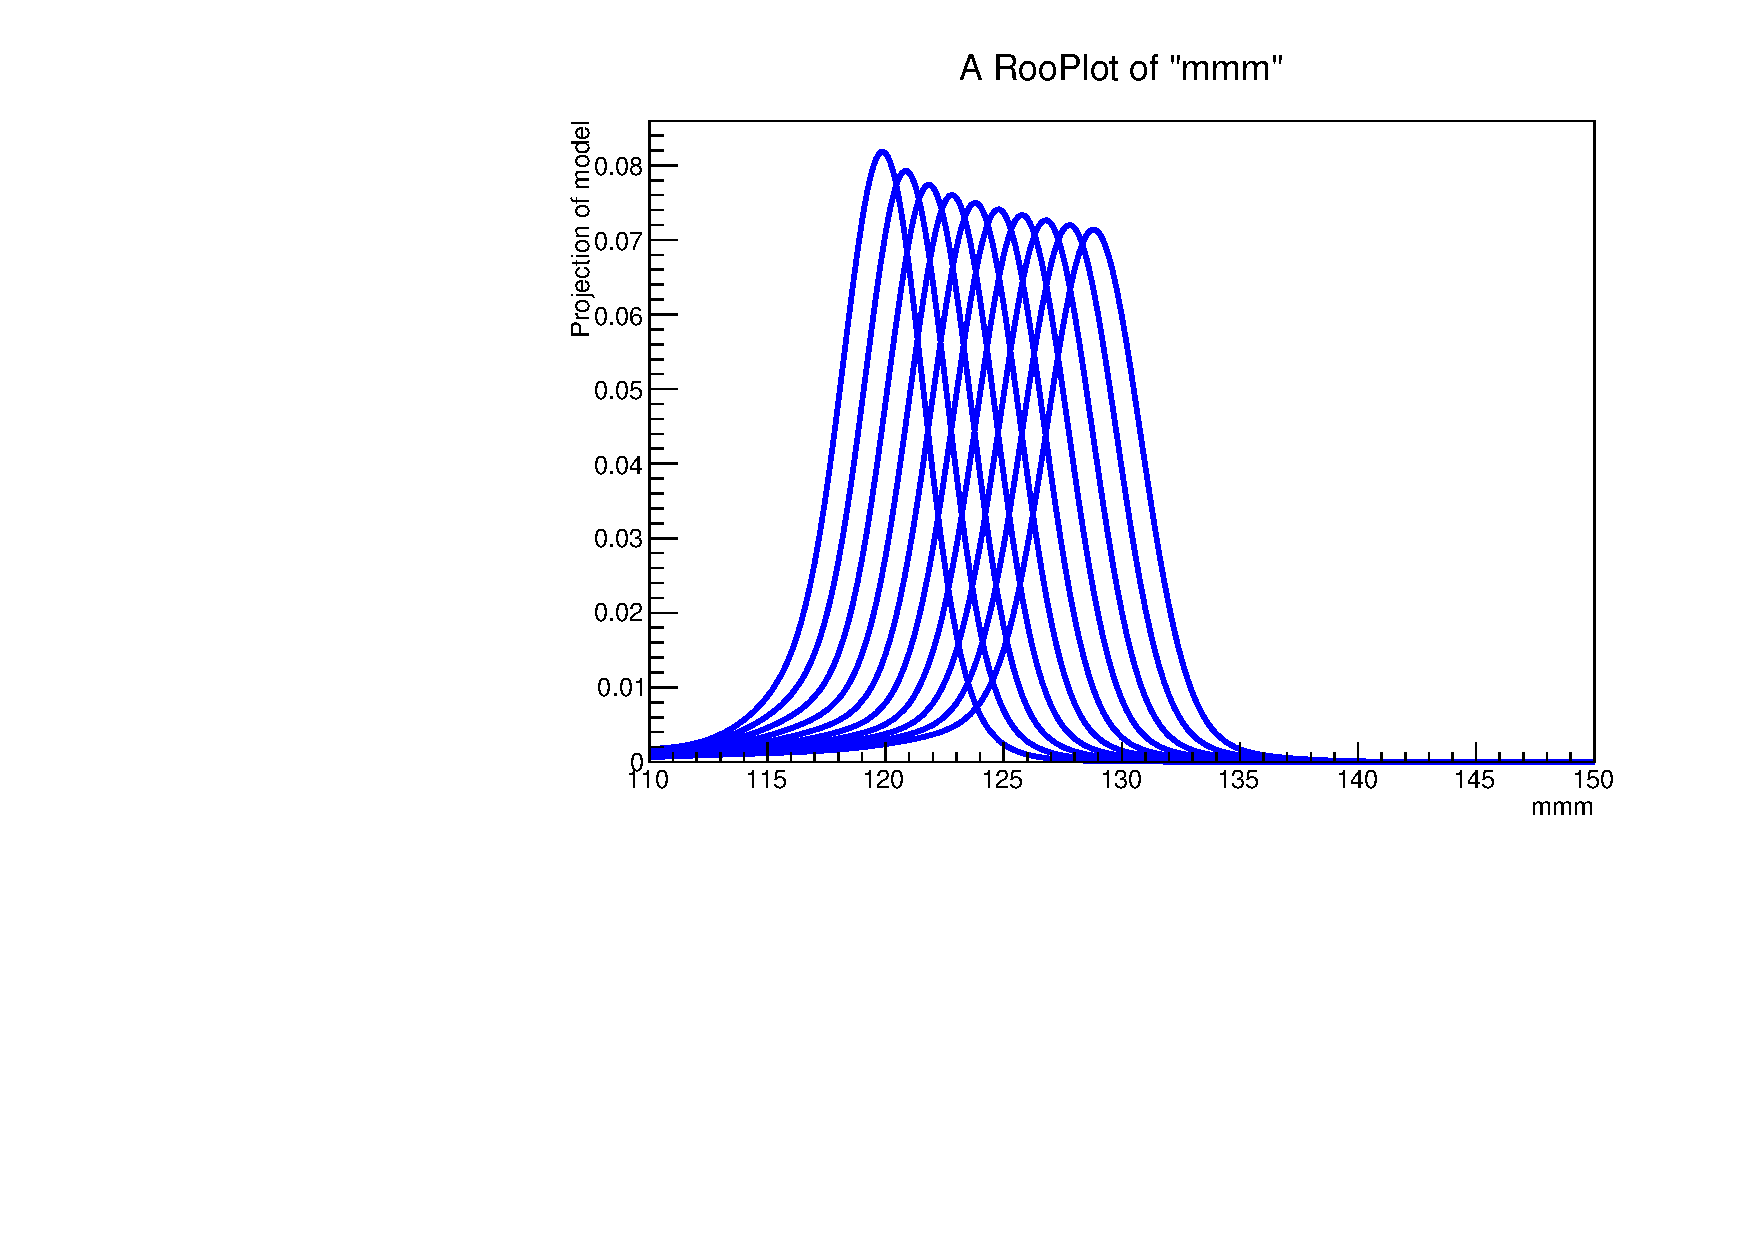
\includegraphics[width=0.49\linewidth]{figures/signal_model/AppendixBdt/interpolation_VBF_cat10.pdf}\\
  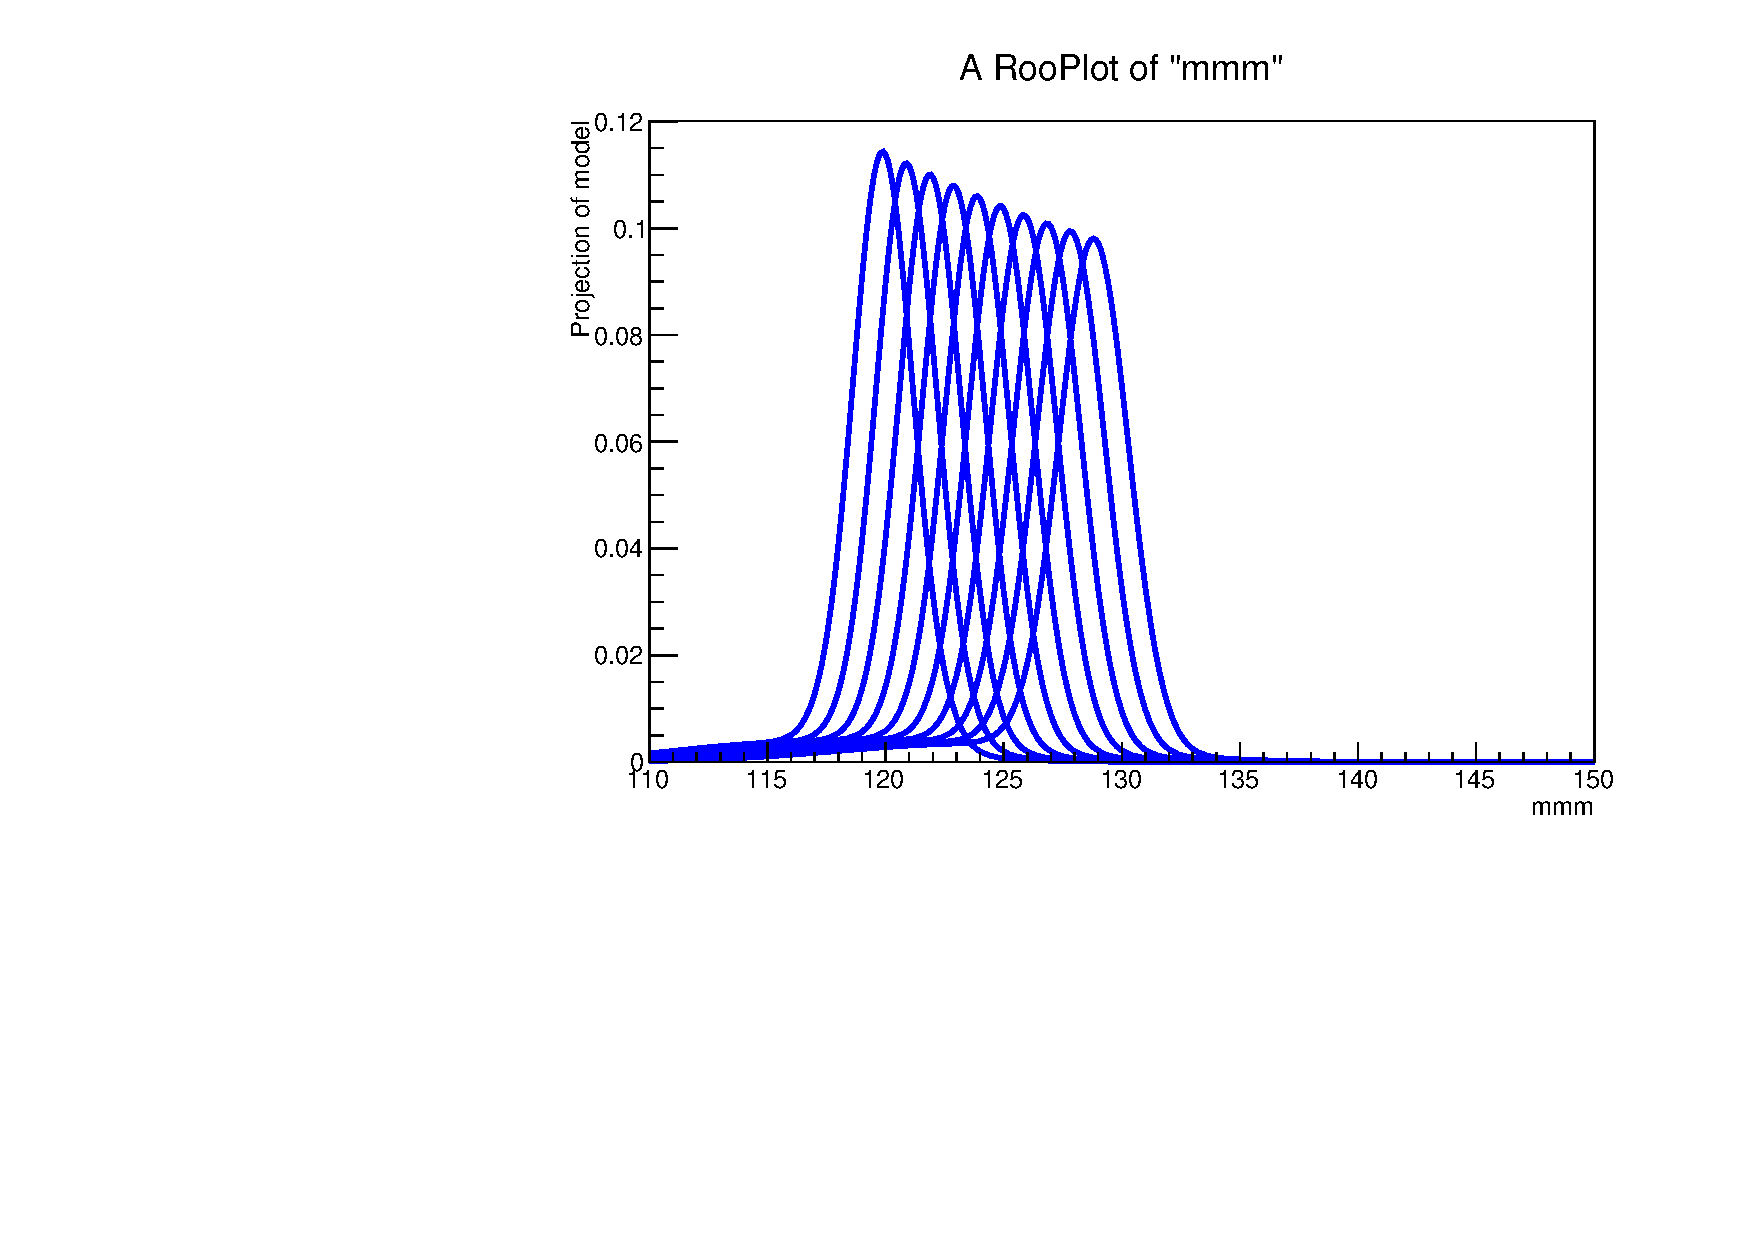
\includegraphics[width=0.49\linewidth]{figures/signal_model/AppendixBdt/interpolation_GluGlu_cat11.pdf}
  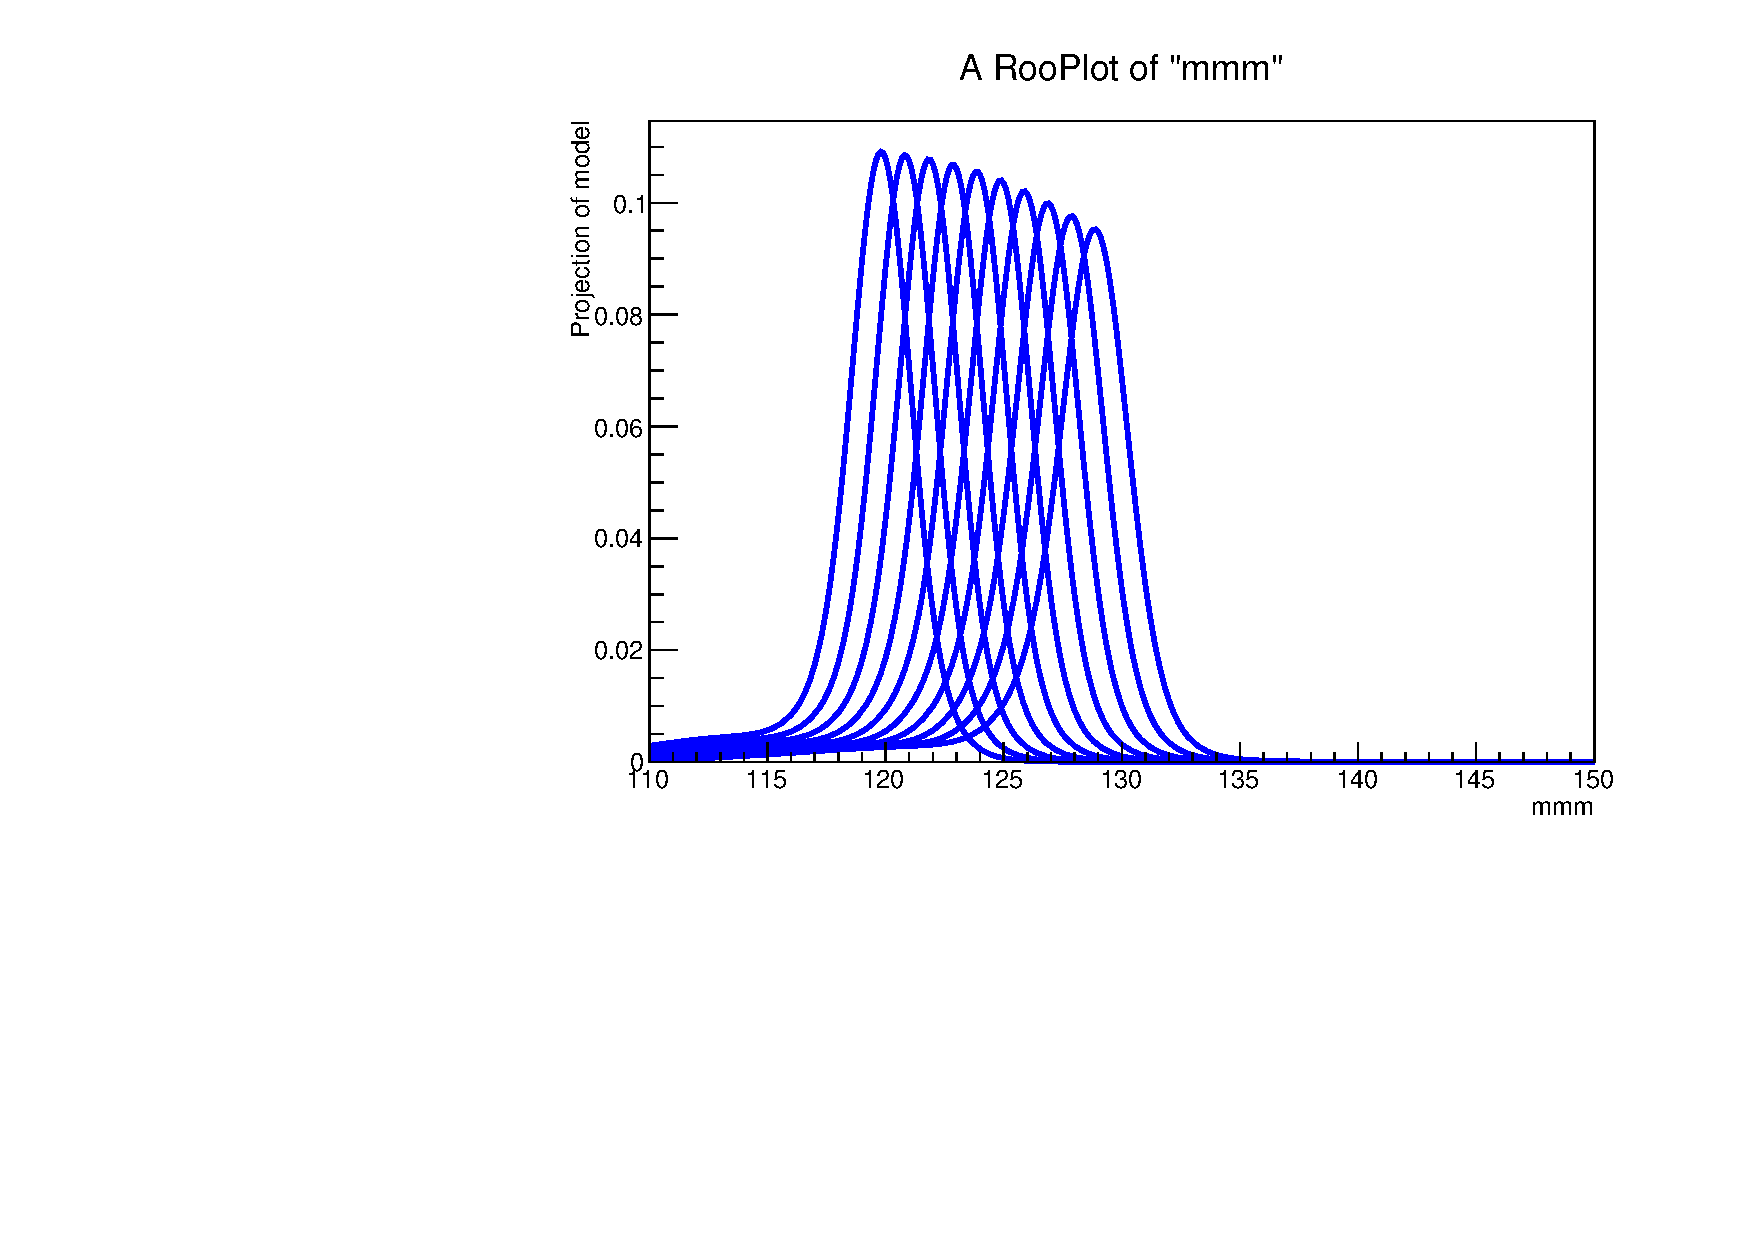
\includegraphics[width=0.49\linewidth]{figures/signal_model/AppendixBdt/interpolation_VBF_cat11.pdf}
  \caption{Signal Model Interpolation. Gluon Fusion (left column) and Vector Boson Fusion (right column). ''c9'' (top row), ''c10'' (middle row) and ''c11'' (bottom row)}
  \label{fig:higgs_signalmodel_gluvbfc9c11}
\end{figure}
%whose entries correspond to the weighted number of events ($\rm{N_{i}}$) per bin,
%the overall normalization is computed according to eq~\ref{eq:signalNormalization}.
%which we can rewrite in terms of efficience and acceptance as in eq~\ref{eq:efficienceAcceptance}.

%Eq~\ref{eq:efficienceAcceptance} demonstrates three different pieces that will come together later on in section~\ref{combine_tool} : Integrated Luminosity, Cross-Section ($\sigma$) and Branching Ratio, and $\epsilon A$.
%For the purpose of modeling, Integrated Luminosity is a single number that is measured centrally; $\epsilon A$ is the normalization we extract from SM Signal Samples and they come in as functions of $\rm{m_{H}}$. Finally, for Cross-Sections and Branching Ratios, which are also functions of $\rm{m_{H}}$, we use centrally provided values by Combine (see more on this in section~\ref{combine_tool}).

% Figure~\ref{sigmodel:comp} shows the composition of the signal model in the different categories of the ``Bdt'' analysis, and the total efficiency times acceptance of the selection prior to categorization.

% \begin{figure}[hbp]
%     \centering
%     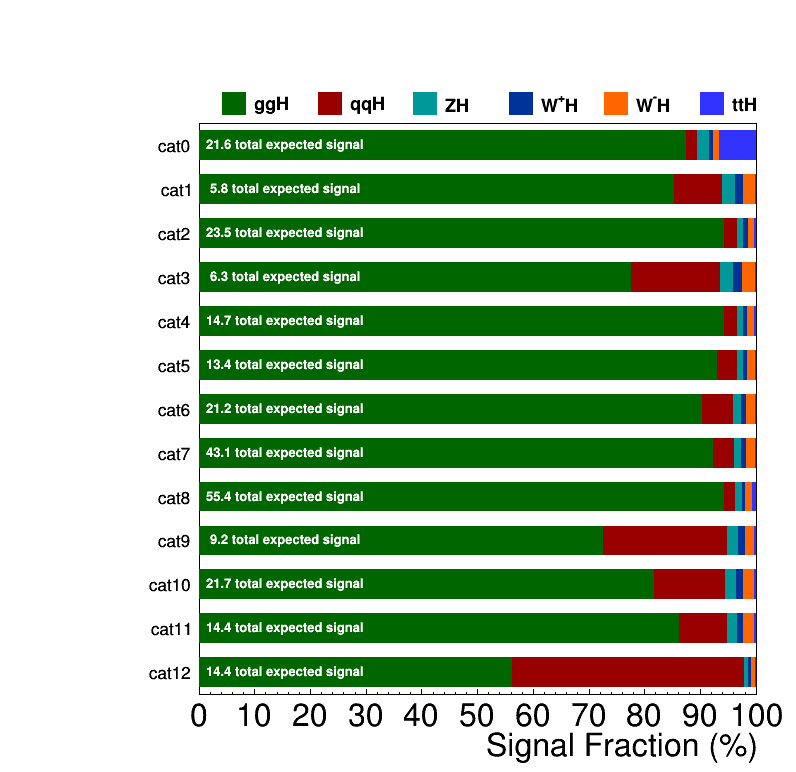
\includegraphics[width=0.49\textwidth]{figures/signal_model/signal_composition}
%     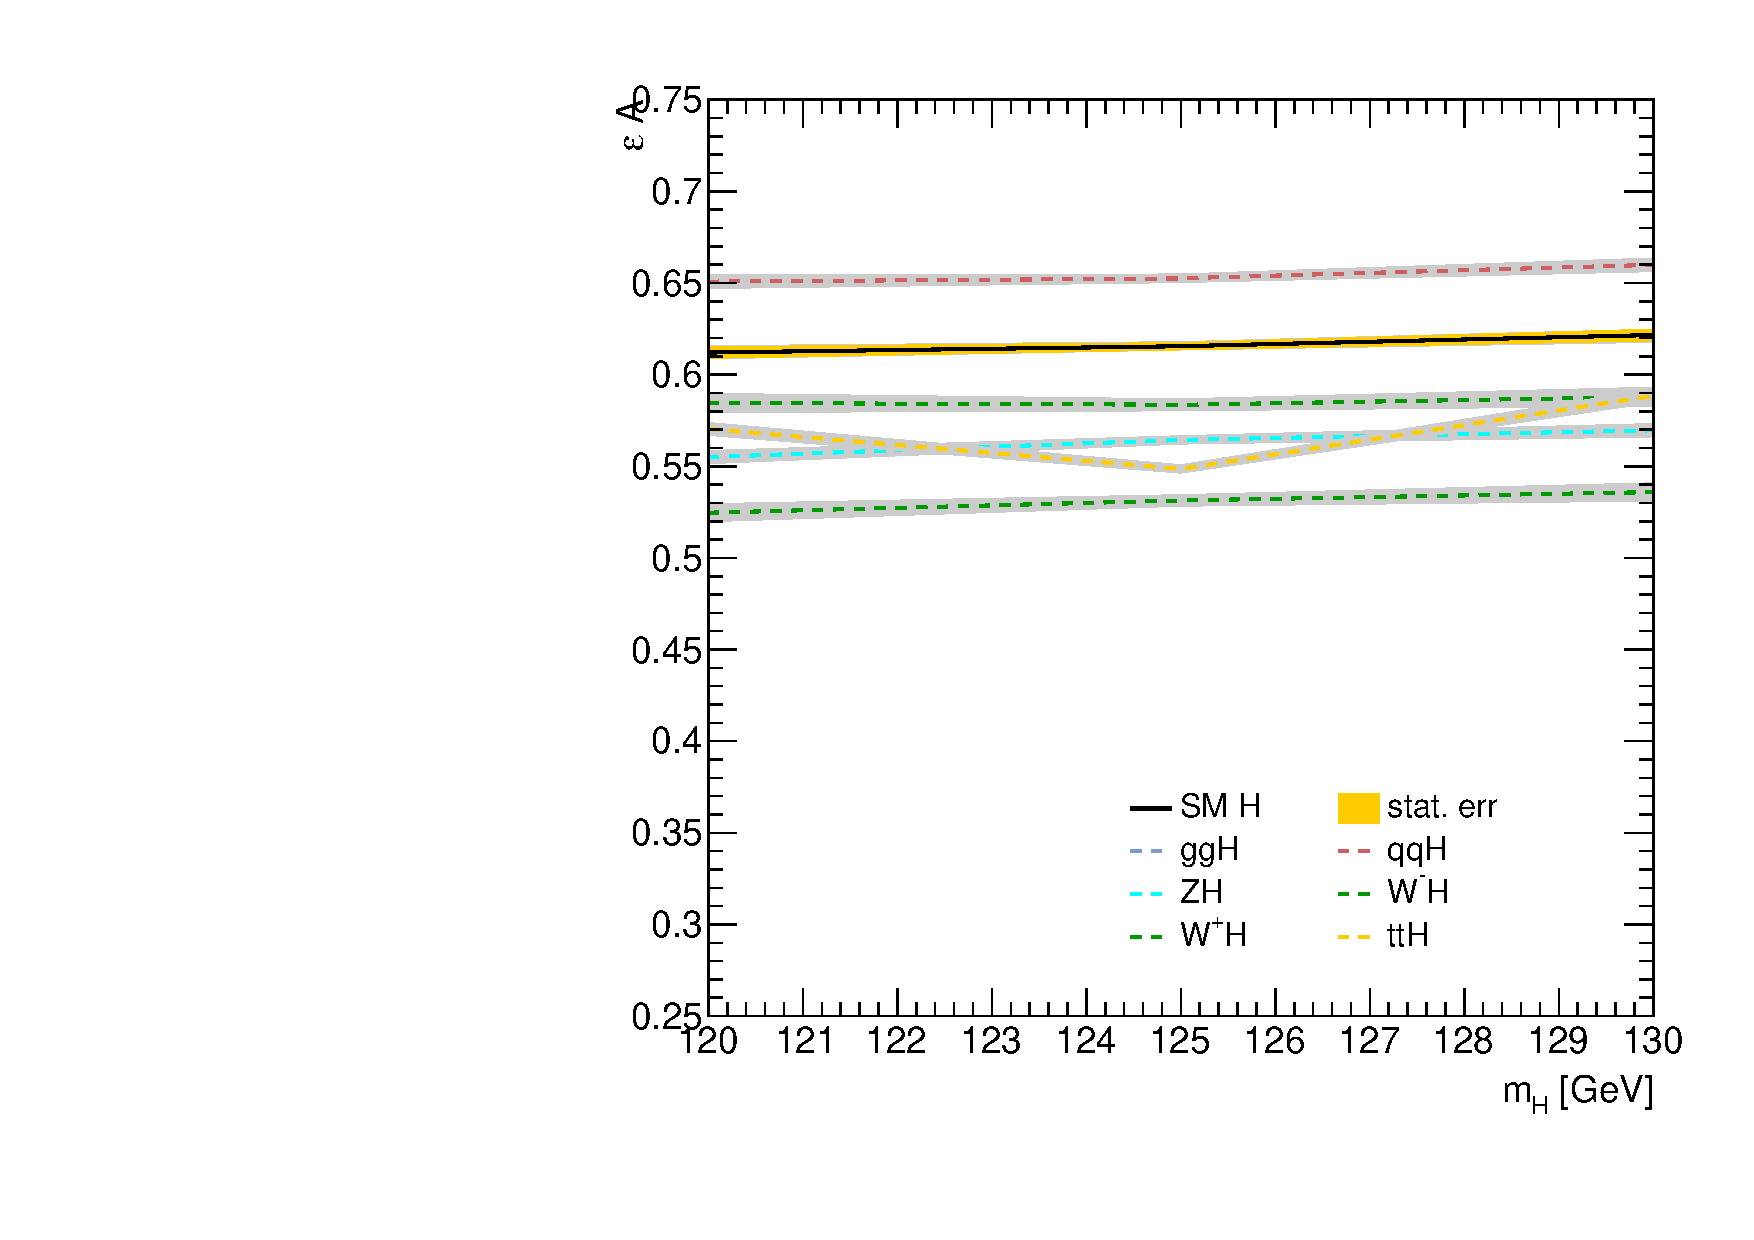
\includegraphics[width=0.49\textwidth]{figures/signal_model/effAcc}
%     \caption{Left: Composition of the different categories of the ``Bdt'' analysis and expected yields of signal events.
%     Right: Efficiency times acceptance of the total selection as function of \mH.}
%     \label{sigmodel:comp}
% \end{figure}

